\documentclass[11pt,letterpaper]{article}


% pmml  arff  openannotation

%\usepackage[condensed,math]{anttor}
%\usepackage[T1]{fontenc}

%\usepackage[T1]{fontenc}
%\usepackage{tgtermes}

\usepackage[hang,flushmargin]{footmisc}

\usepackage{titlesec}

%\usepackage{sectsty}
%\sectionfont{\fontsize{13}{4}\selectfont}

\titleformat{\section}
  {\normalfont\fontsize{13}{15}\bfseries}{\thesection}{1em}{}

\let\OldPart\part

\renewcommand{\part}[1]{\OldPart{#1}%
%{\textcolor{darkRed}\hrule}
\vspace{-.5em}}

\titlespacing*{\section}
{0pt}{4.1ex plus 1ex minus .1ex}{-0.2ex plus .2ex}

\titlespacing*{\subsection}
{0pt}{3.1ex plus 1ex minus .1ex}{-.8ex plus .2ex}

%\usepackage{mathptmx}

\usepackage{eso-pic}

%\setlength\parindent{0pt}

\AddToShipoutPictureBG{%

\ifnum\value{page}>1{
\AtTextUpperLeft{
\makebox[20.5cm][r]{
\raisebox{-2.45cm}{%
{\transparent{0.3}{
\includegraphics[width=0.29\textwidth]{e-logo.png}}	}} } }
}\fi
}

\AddToShipoutPicture{%
{
 {\color{blGreen!70!red}\transparent{0.9}{\put(0,0){\rule{3pt}{\paperheight}}}}%
 {\color{darkRed!70!purple}\transparent{1}\put(3,0){{\rule{4pt}{\paperheight}}}}
% {\color{logoPeach!80!cyan}\transparent{0.5}{\put(0,700){\rule{1cm}{.6cm}}}}%
% {\color{darkRed!60!cyan}\transparent{0.7}\put(0,706){{\rule{1cm}{.6cm}}}}
% \put(18,726){\thepage}
% \transparent{0.8}
}
}

\AddToShipoutPicture{%
\ifnum\value{page}=1
\put(257.5,942){%
	\transparent{0.7}{
		
\includegraphics[width=0.2\textwidth]{logo.png}}}
\put(59,953){\textbf{{\fontfamily{phv}\fontsize{14}{14}\selectfont{}WHITE PAPER}}}
\fi
}	



\AddToShipoutPicture{%
\ifnum\value{page}>1
{\color{blGreen!70!red}\transparent{0.9}{\put(300,6){\rule{0.5\paperwidth}{.3cm}}}}%
{\color{inOne}\transparent{0.8}{\put(300,8){\rule{0.5\paperwidth}{.3cm}}}}%
{\color{inTwo}\transparent{0.3}\put(300,11){{\rule{0.5\paperwidth}{.3cm}}}}

\put(301,14){%
\transparent{0.7}{

\includegraphics[width=0.2\textwidth]{logo.png}}
}
%\fi

%\pgfmathparse{equal(\value{page},15)||equal(\value{page},20)?int(1):int(0)}

\ifnum\value{page}=12   %\pgfmathresult>0\relax
\put(232,113){
 {\setlength{\fboxsep}{.65em}\fontsize{9}{10}\selectfont

   {\color{white}{\parbox{11cm}{\vspace{7pt}{\begin{minipage}{.46\textwidth}
	  {\color{black}{\textit{For more information please contact:}}\\\textbf{\color{blGreen!40!blbl}{Amy Neustein, Ph.D., Founder and CEO}}\\  
       \textbf{{\color{blGreen!20!black}Linguistic Technology Systems \\
      amy.neustein@verizon.net \textbullet{} \textbf{(917) 817-2184} }}}
	 \end{minipage}}}}}}
}
\fi

{\color{blGreen!70!red}\transparent{0.9}{\put(5.6,3){\rule{0.5\paperwidth}{.4cm}}}}%
{\color{inOne}\transparent{1}{\put(5.6,8){\rule{0.5\paperwidth}{.4cm}}}}%
{\color{inTwo}\transparent{0.3}\put(5.6,13){{\rule{0.5\paperwidth}{.4cm}}}}

\fi
}

%\pagestyle{empty} % no page number
%\parskip 7.2pt    % space between paragraphs
%\parindent 12pt   % indent for new paragraph
%\textwidth 4.5in  % width of text
%\columnsep 0.8in  % separation between columns

%\setlength{\footskip}{7pt}

\usepackage[paperheight=14in,paperwidth=8.5in]{geometry}
\geometry{left=.72in,top=.39in,right=.68in,bottom=1.14in} %margins

\usepackage{etoolbox}% http://ctan.org/pkg/etoolbox
\makeatletter
% \patchcmd{<cmd>}{<search>}{<replace>}{<success>}{<failure>}
\patchcmd{\@part}{\par}{\quad}{}{}
\patchcmd{\@part}{\huge}{\Large}{}{}
\makeatother

\renewcommand{\partname}{\hspace{-1em}Part}

\renewcommand*\thepart{\Roman{part}:}

\renewcommand{\thepage}{\raisebox{2pt}{\arabic{page}}}

\renewcommand{\footnoterule}{%
	\kern 2pt
	\hrule width .92\textwidth height .5pt
	\kern 6pt
}


\usepackage[hyphens]{url}
\newcommand{\biburl}[1]{ {\fontfamily{gar}\selectfont{\textcolor[rgb]{.2,.6,0}%
{\scriptsize {\url{#1}}}}}}

%\linespread{1.3}

\newcommand{\sectsp}{\vspace{12pt}}

\usepackage{graphicx}
\usepackage{color,framed}

\usepackage{textcomp}

\usepackage{float}

\usepackage{mdframed}


\usepackage{setspace}
\newcommand{\rpdfNotice}[1]{\begin{onehalfspacing}{

\Large #1

}\end{onehalfspacing}}

\usepackage{xcolor}

\usepackage[hyphenbreaks]{breakurl}
\usepackage[hyphens]{url}

\usepackage{hyperref}
%\newcommand{\rpdfLink}[1]{\href{#1}{\small{#1}}}
%\newcommand{\dblHref}[1]{\href{#1}{\small{\burl{#1}}}}
%\newcommand{\browseHref}[2]{\href{#1}{\Large #2}}

\colorlet{blCyan}{cyan!50!blue}

\definecolor{darkRed}{rgb}{.2,.0,.1}


\definecolor{blGreen}{rgb}{.2,.7,.3}

\definecolor{darkBlGreen}{rgb}{.1,.3,.2}

\definecolor{oldBlColor}{rgb}{.2,.7,.3}

\definecolor{blColor}{rgb}{.1,.3,.2}

\definecolor{elColor}{rgb}{.2,.1,0}
\definecolor{flColor}{rgb}{0.7,0.3,0.3}

\definecolor{logoOrange}{RGB}{108, 18, 30}
\definecolor{logoGreen}{RGB}{85, 153, 89}
\definecolor{logoPurple}{RGB}{200, 208, 30}

\definecolor{logoBlue}{RGB}{4, 2, 25}
\definecolor{logoPeach}{RGB}{255, 159, 102}
\definecolor{logoCyan}{RGB}{66, 206, 244}
\definecolor{logoRed}{rgb}{.3,0,0}

\newcommand{\colorq}[1]{{\color{logoOrange!70!black}{\q{\small\textbf{#1}}}}}

\definecolor{inOne}{rgb}{0.122, 0.435, 0.698}% Rule colour
\definecolor{inTwo}{rgb}{0.122, 0.698, 0.435}% Rule colour

\definecolor{outOne}{rgb}{0.435, 0.698, 0.122}% Rule colour
\definecolor{outTwo}{rgb}{0.698, 0.435, 0.122}% Rule colour

\colorlet{linkcolor}{flColor!60!red}


\hypersetup{
	colorlinks=true,
	citecolor=blCyan!40!green,
	filecolor=magenta!30!logoBlue,
	urlcolor=blue,
    linkcolor=linkcolor!70!black,
%    allcolors=blCyan!40!green
}


\usepackage[many]{tcolorbox}% http://ctan.org/pkg/tcolorbox

\usepackage{transparent}

\newlength{\bsep}
\setlength{\bsep}{-1pt}
\let\xbibitem\bibitem
\renewcommand{\bibitem}[2]{\vspace{\bsep}\xbibitem{#1}{#2}}

\newenvironment{cframed}{\begin{mdframed}[linecolor=logoPeach,linewidth=0.4mm]}{\end{mdframed}}

\newenvironment{ccframed}{\begin{mdframed}[backgroundcolor=logoGreen!5,linecolor=logoCyan!50!black,linewidth=0.4mm]}{\end{mdframed}}


%\usepackage[T1]{fontenc}

%\usepackage{aurical}
% \Fontauri

\usepackage{gfsdidot}
\usepackage[T1]{fontenc}

%\makeatletter
%\f@family,  cmr, T1, n, m,
%\f@encoding,
%\f@shape,
%\f@series,
%\makeatother



%\usepackage{LibreBodoni}

%\usepackage{fontspec}
%\setmainfont{QTBengal}

\usepackage{relsize}

%
%\newcommand{\bref}[1]{\hspace*{1pt}\textbf{\ref{#1}}}

\newcommand{\bref}[1]{\hspace*{1pt}\textbf{\ref{#1}}}

\newcommand{\pseudoIndent}{

\vspace{10pt}\hspace*{12pt}}

\newcommand{\YPDFI}{{\fontfamily{fvs}\selectfont YPDF-Interactive}}

%
\newcommand{\deconum}[1]{{\protect\raisebox{-1pt}{{\LARGE #1}}}}

\newcommand{\visavis}{vis-\`a-vis}

\newcommand{\VersatileUX}{{\color{red!85!black}{\Fontauri Versatile}}%
{{\fontfamily{qhv}\selectfont\smaller UX}}}

\newcommand{\NDPCloud}{{\color{red!15!black}%
{\fontfamily{qhv}\selectfont {\smaller NDP C{\smaller LOUD}}}}}

\newcommand{\MThreeK}{{\color{blGreen!45!black}%
{\fontfamily{qhv}\fontsize{10}{8}\selectfont {M3K}}}}


\newcommand{\lfNDPCloud}{{\color{red!15!black}%
{\fontfamily{qhv}\selectfont N{\smaller DP C{\smaller LOUD}}}}}

\newcommand{\textds}[1]{{\fontfamily{lmdh}\selectfont{%
\raisebox{-1pt}{#1}}}}

\newcommand{\dsC}{{\textds{ds}{\fontfamily{qhv}\selectfont \raisebox{-1pt}
{\color{red!15!black}{C}}}}}

\definecolor{tcolor}{RGB}{24,52,61}

\newcommand{\CCpp}{\resizebox{!}{7pt}{\AcronymText{C}}/\Cpp{}}
\newcommand{\NoSQL}{\resizebox{!}{7pt}{\AcronymText{NoSQL}}}
\newcommand{\SQL}{\resizebox{!}{7pt}{\AcronymText{SQL}}}

\newcommand{\SPARQL}{\resizebox{!}{7pt}{\AcronymText{SPARQL}}}

\newcommand{\NCBI}{\resizebox{!}{7pt}{\AcronymText{NCBI}}}

\newcommand{\HTXN}{\resizebox{!}{7pt}{\ATexttclr{HTXN}}}

\newcommand{\sHTXN}{\resizebox{!}{6pt}{\ATexttclr{HTXN}}}

\newcommand{\TDM}{\resizebox{!}{7pt}{\AcronymText{TDM}}}

\newcommand{\lHTXN}{\resizebox{!}{7.5pt}{\ATexttclr{H}}%
\resizebox{!}{6.5pt}{\ATexttclr{TXN}}}

\newcommand{\lsHTXN}{\resizebox{!}{9.5pt}{\ATexttclr{HTXN}}}

\newcommand{\LAF}{\resizebox{!}{7pt}{\AcronymText{LAF}}}

\newcommand{\UDpipe}{\resizebox{!}{7pt}{\AcronymText{UDpipe}}}

\newcommand{\C}{\resizebox{!}{7pt}{\AcronymText{C}}}

\newcommand{\FCS}{\resizebox{!}{7pt}{\AcronymText{FCS}}}

\newcommand{\GAVI}{\resizebox{!}{7pt}{\AcronymText{GAVI}}}
\newcommand{\ArcGIS}{\resizebox{!}{7pt}{\AcronymText{ArcGIS}}}
\newcommand{\QGIS}{\resizebox{!}{7pt}{\AcronymText{QGIS}}}

\newcommand{\GIS}{\resizebox{!}{7pt}{\AcronymText{GIS}}}
\newcommand{\AngelScript}{\resizebox{!}{7pt}{\AcronymText{AngelScript}}}



\usepackage{mdframed}

\newcommand{\cframedboxpanda}[1]{\begin{mdframed}[linecolor=yellow!70!blue,linewidth=0.4mm]#1\end{mdframed}}


\newcommand{\PVD}{\resizebox{!}{7pt}{\AcronymText{PVD}}}

\newcommand{\TAGML}{\resizebox{!}{7pt}{\AcronymText{TAGML}}}
\newcommand{\sTAGML}{\resizebox{!}{6pt}{\AcronymText{TAGML}}}

\newcommand{\GTagML}{\resizebox{!}{7pt}{\ATexttclr{G{%
\scriptsize{TAG}}ML}}}

\newcommand{\lGTagML}{\resizebox{!}{7.5pt}{\ATexttclr{G{%
\scriptsize{TAG}}ML}}}

\newcommand{\SDK}{\resizebox{!}{7pt}{\AcronymText{SDK}}}
\newcommand{\NLP}{\resizebox{!}{7pt}{\AcronymText{NLP}}}

\newcommand{\AXF}{\resizebox{!}{7pt}{\ATexttclr{AXF}}}

\newcommand{\HyperGraphDB}{\resizebox{!}{7pt}{\AcronymText{HyperGraphDB}}}

\newcommand{\AllegroGraph}{\resizebox{!}{7pt}{\AcronymText{AllegroGraph}}}

\newcommand{\Grakenai}{\resizebox{!}{7pt}{\AcronymText{Graken.ai}}}


\newcommand{\lAXF}{\resizebox{!}{7.5pt}{\ATexttclr{A}}%
\resizebox{!}{6.5pt}{\ATexttclr{XF}}}


\newcommand{\lsAXF}{\resizebox{!}{8.5pt}{\ATexttclr{AXF}}}

\newcommand{\AXFD}{\resizebox{!}{7pt}{\ATexttclr{AXFD}}}

\newcommand{\CBICA}{\resizebox{!}{7pt}{\AcronymText{CBICA}}}

\newcommand{\IORT}{\resizebox{!}{7pt}{\AcronymText{IORT}}}

\newcommand{\openCyto}{\resizebox{!}{7pt}{\AcronymText{openCyto}}}
\newcommand{\FACSanadu}{\resizebox{!}{7pt}{\AcronymText{FACSanadu}}}
\newcommand{\cytoLib}{\resizebox{!}{7pt}{\AcronymText{cytoLib}}}


\newcommand{\sopenCyto}{\resizebox{!}{6pt}{\AcronymText{openCyto}}}
\newcommand{\sFACSanadu}{\resizebox{!}{6pt}{\AcronymText{FACSanadu}}}
\newcommand{\scytoLib}{\resizebox{!}{6pt}{\AcronymText{cytoLib}}}

\newcommand{\sJava}{\resizebox{!}{6pt}{\AcronymText{Java}}}
\newcommand{\sGUI}{\resizebox{!}{6pt}{\AcronymText{GUI}}}
\newcommand{\sCpp}{\resizebox{!}{6pt}{\AcronymText{C++}}}
\newcommand{\sR}{\resizebox{!}{6pt}{\AcronymText{R}}}
\newcommand{\sQt}{\resizebox{!}{6pt}{\AcronymText{Qt}}}


\newcommand{\SeDI}{\resizebox{!}{7pt}{\AcronymText{SeDI}}}
\newcommand{\RSNA}{\resizebox{!}{7pt}{\AcronymText{RSNA}}}

\newcommand{\CER}{\resizebox{!}{7pt}{\AcronymText{CER}}}
\newcommand{\PACS}{\resizebox{!}{7pt}{\AcronymText{PACS}}}

\newcommand{\DCMTK}{\resizebox{!}{7pt}{\AcronymText{DCMTK}}}
\newcommand{\lsDCMTK}{\resizebox{!}{9pt}{\AcronymText{DCMTK}}}

\newcommand{\DICOM}{\resizebox{!}{7pt}{\AcronymText{DICOM}}}
\newcommand{\lsDICOM}{\resizebox{!}{9pt}{\AcronymText{DICOM}}}

\newcommand{\CytometryML}{\resizebox{!}{7pt}{\AcronymText{CytometryML}}}

\newcommand{\FCM}{\resizebox{!}{7pt}{\AcronymText{FCM}}}

\newcommand{\OMETIFF}{\resizebox{!}{7pt}{\AcronymText{OME-TIFF}}}
\newcommand{\OME}{\resizebox{!}{7pt}{\AcronymText{OME}}}

\newcommand{\sOMETIFF}{\resizebox{!}{6pt}{\AcronymText{OME-TIFF}}}
\newcommand{\sOME}{\resizebox{!}{6pt}{\AcronymText{OME}}}

\newcommand{\sXML}{\resizebox{!}{6pt}{\AcronymText{XML}}}

\newcommand{\CT}{\resizebox{!}{7pt}{\AcronymText{CT}}}

\newcommand{\LOINC}{\resizebox{!}{7pt}{\AcronymText{LOINC}}}

\newcommand{\RadLex}{\resizebox{!}{7pt}{\AcronymText{RadLex}}}

\newcommand{\DCC}{\resizebox{!}{7pt}{\AcronymText{DCC}}}


\newcommand{\OMOP}{\resizebox{!}{7pt}{\AcronymText{OMOP}}}
\newcommand{\PCORnet}{\resizebox{!}{7pt}{\AcronymText{PCORnet}}}
\newcommand{\FHIR}{\resizebox{!}{7pt}{\AcronymText{FHIR}}}

\newcommand{\CaPTk}{\resizebox{!}{7pt}{\AcronymText{CaPTk}}}

\newcommand{\WebGL}{\resizebox{!}{7pt}{\AcronymText{WebGL}}}


\newcommand{\VIOLIN}{\resizebox{!}{7pt}{\AcronymText{VIOLIN}}}



\newcommand{\lAXFD}{\resizebox{!}{7.5pt}{\ATexttclr{A}}%
\resizebox{!}{6.5pt}{\ATexttclr{XFD}}}


\newcommand{\IJST}{\resizebox{!}{7pt}{\AcronymText{IJST}}}

\newcommand{\BioC}{\resizebox{!}{7pt}{\AcronymText{BioC}}}

\newcommand{\CoNLL}{\resizebox{!}{7pt}{\AcronymText{CoNLL}}}
\newcommand{\CoNLLU}{\resizebox{!}{7pt}{\AcronymText{CoNLL-U}}}

\newcommand{\sapp}{\resizebox{!}{7pt}{\AcronymText{Sapien+}}}
\newcommand{\lsapp}{\resizebox{!}{8.5pt}{\AcronymText{Sapien+}}}
\newcommand{\lssapp}{\resizebox{!}{9.5pt}{\AcronymText{Sapien+}}}

\newcommand{\ePub}{\resizebox{!}{7pt}{\AcronymText{ePub}}}

%\lsLPF


\newcommand{\GIT}{\resizebox{!}{7pt}{\AcronymText{GIT}}}

%\definecolor{atColor}{RGB}{11, 71, 17}


\DeclareMathVersion{fordg}
\SetSymbolFont{letters}{fordg}{OML}{cmr}{b}{n}

\definecolor{atcColor}{RGB}{96, 17, 12}
%\textcolor{tcolor}{

\newcommand{\ATextCClr}[1]{\textcolor{atcColor}{\textbf{#1}}}

\newcommand{\ATexttclr}[1]{\textcolor{tcolor}{\textbf{#1}}}

\newcommand{\AIMConc}{\resizebox{!}{7.5pt}{\ATextCClr{AIM-Concepts}}}
\newcommand{\lAIMConc}{\resizebox{!}{8pt}{\ATextCClr{AIM-Concepts}}}

\newcommand{\HGXF}{{\resizebox{!}{7.5pt}{\ATexttclr{HGXF}}}}
\newcommand{\lHGXF}{{\resizebox{!}{8pt}{\ATexttclr{HGXF}}}}
\newcommand{\sHGXF}{{\resizebox{!}{6pt}{\ATexttclr{HGXF}}}}

\newcommand{\CRtwo}{{\resizebox{!}{7.5pt}{\ATextCClr{CR2}}}}
\newcommand{\lCRtwo}{{\resizebox{!}{8pt}{\ATextCClr{CR2}}}}
\newcommand{\sCRtwo}{{\resizebox{!}{6pt}{\ATextCClr{CR2}}}}



\newcommand{\THQL}{\resizebox{!}{7.5pt}{\ATexttclr{THQL}}}
\newcommand{\lTHQL}{\resizebox{!}{8pt}{\ATexttclr{THQL}}}

\newcommand{\HDICOM}{\resizebox{!}{7.5pt}{\ATexttclr{{\large h}-DICOM}}}

\newcommand{\hVaImm}{\resizebox{!}{7.5pt}{\ATexttclr{{\large h}-VaImm}}}


\newcommand{\PhaonVI}{\resizebox{!}{7.5pt}{\ATexttclr{Phaon-VI}}}



\definecolor{atColor}{RGB}{50, 22, 40}
\newcommand{\ATextClr}[1]{\textcolor{atColor}{\textbf{#1}}}

\newcommand{\DgDb}{{\mathversion{fordg}%
\makebox{\raisebox{-3pt}{\resizebox{!}{11pt}{\ATextClr{%
\rotatebox{17}{$\varsigma$}}}}\hspace{-4pt}%
\resizebox{!}{6.5pt}{\ATextClr{D\hspace{-2pt}B}}}}}


\newcommand{\lDgDb}{{\mathversion{fordg}%
\resizebox{!}{12pt}{\ATextClr{%
\rotatebox{17}{$\varsigma$}}}}\hspace{-4pt}%
\resizebox{!}{6.5pt}{\ATextClr{D\hspace{-2pt}B}}}}}

\newcommand{\URL}{\resizebox{!}{7pt}{\AcronymText{URL}}}
\newcommand{\CSML}{\resizebox{!}{7pt}{\AcronymText{CSML}}}
\newcommand{\LPF}{\resizebox{!}{7pt}{\AcronymText{LPF}}}
\newcommand{\lLPF}{\resizebox{!}{8.5pt}{\AcronymText{LPF}}}
\newcommand{\lsLPF}{\resizebox{!}{9.5pt}{\AcronymText{LPF}}}

\newcommand{\AI}{\resizebox{!}{7.5pt}{\AcronymText{AI}}}
\newcommand{\lAI}{\resizebox{!}{8pt}{\AcronymText{AI}}}

\newcommand{\Jupyter}{\resizebox{!}{7pt}{\AcronymText{Jupyter}}}
\newcommand{\Python}{\resizebox{!}{7pt}{\AcronymText{Python}}}
\newcommand{\IDN}{\resizebox{!}{7pt}{\AcronymText{IDN}}}
\newcommand{\JPG}{\resizebox{!}{7pt}{\AcronymText{JPG}}}
\newcommand{\JPEG}{\resizebox{!}{7pt}{\AcronymText{JPEG}}}
\newcommand{\PNG}{\resizebox{!}{7pt}{\AcronymText{PNG}}}
\newcommand{\TIFF}{\resizebox{!}{7pt}{\AcronymText{TIFF}}}
\newcommand{\REPL}{\resizebox{!}{7pt}{\AcronymText{REPL}}}

\newcommand{\Pandore}{\resizebox{!}{7pt}{\AcronymText{Pandore}}}

\newcommand{\MIFlowCyt}{\resizebox{!}{7pt}{\AcronymText{MIFlowCyt}}}
\newcommand{\GatingML}{\resizebox{!}{7pt}{\AcronymText{Gating-ML}}}
\newcommand{\flowCL}{\resizebox{!}{7pt}{\AcronymText{flowCL}}}


\makeatletter

\newcommand*\getX[1]{\expandafter\getX@i#1\@nil}

\newcommand*\getY[1]{\expandafter\getY@i#1\@nil}
\def\getX@i#1,#2\@nil{#1}
\def\getY@i#1,#2\@nil{#2}
\makeatother
	
\definecolor{BlueGreen}{rgb}{.1,.6,.4}

\newcommand{\ann}[9]{%
	\path [draw=#1,draw opacity=#2,line width=#3, fill=#4, fill opacity = #5, even odd rule] %
	(#6) ellipse(#7 and #8) ellipse(#7*#9 and #8*#9);}

\newcommand{\rectann}[9]{%
\path [draw=#1,draw opacity=#2,line width=#3, fill=#4, fill opacity = #5, even odd rule] %
(#6) rectangle(\getX{#6}+#7,\getY{#6}+#8)
({\getX{#6}+((#7-(#7*#9))/2)},{\getY{#6}+((#8-(#8*#9))/2)}) rectangle %
({\getX{#6}+((#7-(#7*#9))/2)+#7*#9},{\getY{#6}+((#8-(#8*#9))/2)+#8*#9});}

\definecolor{grammarArrowColor}{rgb}{.85,.85,.45}

\definecolor{pfcolor}{RGB}{94, 54, 73}

\newcommand{\EPF}{\resizebox{!}{7pt}{\AcronymText{ETS{\color{pfcolor}pf}}}}
\newcommand{\lEPF}{\resizebox{!}{8.5pt}{\AcronymText{ETS{\color{pfcolor}pf}}}}
\newcommand{\lsEPF}{\resizebox{!}{9.5pt}{\AcronymText{ETS{\color{pfcolor}pf}}}}


\newcommand{\XPDF}{\resizebox{!}{7pt}{\AcronymText{XPDF}}}

\newcommand{\GRE}{\resizebox{!}{7pt}{\AcronymText{GRE}}}
\newcommand{\CAS}{\resizebox{!}{7pt}{\AcronymText{CAS}}}

\newcommand{\lMOSAIC}{%
\resizebox{!}{8pt}{\ATexttclr{M}}%
\resizebox{!}{6pt}{\ATexttclr{OSAIC}}}

\newcommand{\llMOSAIC}{%
\resizebox{!}{8.5pt}{\ATexttclr{MOSAIC}}}

\newcommand{\ConceptsDB}{\resizebox{!}{7.5pt}{\ATexttclr{ConceptsDB}}}

\newcommand{\sConceptsDB}{\resizebox{!}{7pt}{\ATexttclr{ConceptsDB}}}

\newcommand{\lConceptsDB}{\resizebox{!}{8pt}{\ATexttclr{C}}%
\resizebox{!}{7.5pt}{\ATexttclr{onceptsDB}}}

\newcommand{\llConceptsDB}{\resizebox{!}{8.5pt}{\ATexttclr{C}}%
\resizebox{!}{8pt}{\ATexttclr{onceptsDB}}}

\newcommand{\CsAF}{\resizebox{!}{7pt}{\ATexttclr{CsAF}}}
\newcommand{\lCsAF}{\resizebox{!}{8pt}{\ATexttclr{C}}%
\resizebox{!}{7.5pt}{\ATexttclr{sAF}}}


\newcommand{\XML}{\resizebox{!}{7pt}{\AcronymText{XML}}}

\newcommand{\lXML}{\resizebox{!}{8pt}{\AcronymText{XML}}}

\newcommand{\RDF}{\resizebox{!}{7pt}{\AcronymText{RDF}}}
\newcommand{\DOM}{\resizebox{!}{7pt}{\AcronymText{DOM}}}

\newcommand{\Java}{\resizebox{!}{7pt}{\AcronymText{Java}}}


\newcommand{\ParaView}{\resizebox{!}{7pt}{\AcronymText{ParaView}}}
\newcommand{\Octave}{\resizebox{!}{7pt}{\AcronymText{Octave}}}
\newcommand{\ROOT}{\resizebox{!}{7pt}{\AcronymText{ROOT}}}
\newcommand{\CERN}{\resizebox{!}{7pt}{\AcronymText{CERN}}}
\newcommand{\MQFour}{\resizebox{!}{7pt}{\AcronymText{MQ4}}}
\newcommand{\VISSION}{\resizebox{!}{7pt}{\AcronymText{VISSION}}}

\newcommand{\sVISSION}{\resizebox{!}{6pt}{\AcronymText{VISSION}}}


\newcommand{\ReproZip}{\resizebox{!}{7pt}{\AcronymText{ReproZip}}}
\newcommand{\BioCoder}{\resizebox{!}{7pt}{\AcronymText{BioCoder}}}

\newcommand{\Covid}{\resizebox{!}{7pt}{\AcronymText{Covid-19}}}


\newcommand{\HMCL}{{\resizebox{!}{7.5pt}{\ATexttclr{HMCL}}}}
\newcommand{\DSPIN}{{\resizebox{!}{7.5pt}{\ATexttclr{D-SPIN}}}}

%\newcommand{\Pandore}{{\resizebox{!}{7.5pt}{\ATexttclr{Pandore}}}}

\newcommand{\lDSPIN}{{\resizebox{!}{8pt}{\ATexttclr{D-SPIN}}}}
\newcommand{\lsDSPIN}{{\resizebox{!}{8.5pt}{\ATexttclr{D-SPIN}}}}

\newcommand{\CLang}{\resizebox{!}{7pt}{\AcronymText{C}}}

\newcommand{\HNaN}{\resizebox{!}{7pt}{\AcronymText{HN%
\textsc{a}N}}}

\newcommand{\JSON}{\resizebox{!}{7pt}{\AcronymText{JSON}}}
\newcommand{\UV}{\resizebox{!}{7pt}{\AcronymText{UV}}}

\newcommand{\sJSON}{\resizebox{!}{6pt}{\AcronymText{JSON}}}

\newcommand{\PET}{\resizebox{!}{7pt}{\AcronymText{PET}}}
\newcommand{\MRI}{\resizebox{!}{7pt}{\AcronymText{MRI}}}


\newcommand{\MeshLab}{\resizebox{!}{7pt}{\AcronymText{MeshLab}}}
\newcommand{\IQmol}{\resizebox{!}{7pt}{\AcronymText{IQmol}}}

\newcommand{\SGML}{\resizebox{!}{7pt}{\AcronymText{SGML}}}

\newcommand{\WhiteDB}{\resizebox{!}{7pt}{\AcronymText{\makebox{WhiteDB}}}}

\newcommand{\CrossRef}{\resizebox{!}{7pt}{\AcronymText{CrossRef}}}

\newcommand{\ASCII}{\resizebox{!}{7pt}{\AcronymText{ASCII}}}

\newcommand{\GUI}{\resizebox{!}{7pt}{\AcronymText{GUI}}}
\newcommand{\UI}{\resizebox{!}{7pt}{\AcronymText{UI}}}


\newcommand{\URI}{\resizebox{!}{7pt}{\AcronymText{URI}}}
\newcommand{\DTD}{\resizebox{!}{7pt}{\AcronymText{DTD}}}
\newcommand{\sDTD}{\resizebox{!}{6pt}{\AcronymText{DTD}}}

\newcommand{\API}{\resizebox{!}{7pt}{\AcronymText{API}}}

\newcommand{\JATS}{\resizebox{!}{7pt}{\AcronymText{JATS}}}


\newcommand{\SDI}{\resizebox{!}{7pt}{\AcronymText{SDI}}}
\newcommand{\SDIV}{\resizebox{!}{7pt}{\AcronymText{SDIV}}}

\definecolor{atColor}{RGB}{50, 22, 40}
\newcommand{\ATextClr}[1]{\textcolor{atColor}{\textbf{#1}}}

\newcommand{\DgDbx}{\makebox{\raisebox{-3pt}{\resizebox{!}{11pt}{\ATextClr{%
\rotatebox{17}{$\varsigma$}}}}\hspace{-4pt}%
\resizebox{!}{6.5pt}{\ATextClr{D\hspace{-2pt}B}}}}

\newcommand{\lDgDbx}{\makebox{\raisebox{-3pt}{%
\resizebox{!}{12pt}{\ATextClr{%
\rotatebox{17}{$\varsigma$}}}}\hspace{-4pt}%
\resizebox{!}{6.5pt}{\ATextClr{D\hspace{-2pt}B}}}}


\newcommand{\IDE}{\resizebox{!}{7pt}{\AcronymText{IDE}}}

\newcommand{\OWL}{\resizebox{!}{7pt}{\AcronymText{OWL}}}

\newcommand{\Kaggle}{\resizebox{!}{7pt}{\AcronymText{Kaggle}}}


\newcommand{\ViSion}{\resizebox{!}{7pt}{\AcronymText{ViSion}}}

\newcommand{\CWL}{\resizebox{!}{7pt}{\AcronymText{CWL}}}

\newcommand{\ThreeD}{\resizebox{!}{7pt}{\AcronymText{3D}}}
\newcommand{\TwoD}{\resizebox{!}{7pt}{\AcronymText{2D}}}

\newcommand{\medInria}{\resizebox{!}{7pt}{\AcronymText{medInria}}}
\newcommand{\ThreeDimViewer}{\resizebox{!}{7pt}{\AcronymText{3DimViewer}}}

\newcommand{\FAIR}{\resizebox{!}{7pt}{\AcronymText{FAIR}}}

\newcommand{\MIAPEGI}{\resizebox{!}{7pt}{\AcronymText{MIAPE-GI}}}
\newcommand{\MIAPE}{\resizebox{!}{7pt}{\AcronymText{MIAPE}}}



\newcommand{\QNetworkManager}{\resizebox{!}{7pt}{\AcronymText{QNetworkManager}}}
\newcommand{\QTextDocument}{\resizebox{!}{7pt}{\AcronymText{QTextDocument}}}
\newcommand{\QWebEngineView}{\resizebox{!}{7pt}{\AcronymText{QWebEngineView}}}
\newcommand{\HTTP}{\resizebox{!}{7pt}{\AcronymText{HTTP}}}


\newcommand{\lAcronymTextNC}[2]{{\fontfamily{fvs}\selectfont {\Large{#1}}{\large{#2}}}}

\newcommand{\AcronymTextNC}[1]{{\fontfamily{fvs}\selectfont {\large #1}}}


\colorlet{orr}{orange!60!red}

\newcommand{\textscc}[1]{{\color{orr!35!black}{{%
						\fontfamily{Cabin-TLF}\fontseries{b}\selectfont{\textsc{\scriptsize{#1}}}}}}}


\newcommand{\textsccserif}[1]{{\color{orr!35!black}{{%
				\scriptsize{\textbf{#1}}}}}}


\newcommand{\iXPDF}{\resizebox{!}{7pt}{\textsccserif{%
\textit{XPDF}}}}

\newcommand{\iEPF}{\resizebox{!}{7pt}{\textsccserif{%
\textit{ETSpf}}}}

\newcommand{\iSDI}{\resizebox{!}{7pt}{\textsccserif{%
\textit{SDI}}}}

\newcommand{\iHTXN}{\resizebox{!}{7pt}{\textsccserif{%
\textit{HTXN}}}}


\newcommand{\AcronymText}[1]{{\textscc{#1}}}

\newcommand{\AcronymTextser}[1]{{\textsccserif{#1}}}


\newcommand{\mAcronymText}[1]{{\textscc{\normalsize{#1}}}}

\newcommand{\FASTA}{{\resizebox{!}{7pt}{\AcronymText{FASTA}}}}
\newcommand{\SRA}{{\resizebox{!}{7pt}{\AcronymText{SRA}}}}
\newcommand{\DNA}{{\resizebox{!}{7pt}{\AcronymText{DNA}}}}
\newcommand{\MAP}{{\resizebox{!}{7pt}{\AcronymText{MAP}}}}
\newcommand{\EPS}{{\resizebox{!}{7pt}{\AcronymText{EPS}}}}
\newcommand{\CSV}{{\resizebox{!}{7pt}{\AcronymText{CSV}}}}
\newcommand{\PDB}{{\resizebox{!}{7pt}{\AcronymText{PDB}}}}

%\newcommand{\WebGL}{{\resizebox{!}{7pt}{\AcronymText{WebGL}}}}

\newcommand{\Docker}{{\resizebox{!}{7pt}{\AcronymText{Docker}}}}


\newcommand{\OBO}{{\resizebox{!}{7pt}{\AcronymText{OBO}}}}

\newcommand{\XOCS}{{\resizebox{!}{7pt}{\AcronymText{XOCS}}}}

\newcommand{\RNA}{{\resizebox{!}{7pt}{\AcronymText{RNA}}}}

\newcommand{\ChemXML}{{\resizebox{!}{7pt}{\AcronymText{ChemXML}}}}

\newcommand{\TeXMECS}{\resizebox{!}{7pt}{\AcronymText{TeXMECS}}}

% pmml  arff  openannotation

\newcommand{\PMML}{\resizebox{!}{7pt}{\AcronymText{PMML}}}
\newcommand{\ARFF}{\resizebox{!}{7pt}{\AcronymText{ARFF}}}
\newcommand{\IeXML}{\resizebox{!}{7pt}{\AcronymText{IeXML}}}

\newcommand{\SeCo}{\resizebox{!}{7pt}{\AcronymText{SeCo}}}


\newcommand{\HDFFive}{\resizebox{!}{7pt}{\AcronymText{HDF5}}}

\newcommand{\NGML}{\resizebox{!}{7pt}{\ATexttclr{NGML}}}

\newcommand{\SDRM}{\resizebox{!}{7pt}{\ATexttclr{SDRM}}}
\newcommand{\sSDRM}{\resizebox{!}{6pt}{\ATexttclr{SDRM}}}
\newcommand{\lSDRM}{\resizebox{!}{8pt}{\ATexttclr{S}}%
\resizebox{!}{7pt}{\ATexttclr{DRM}}}


%\newcommand{\SDRF}{\resizebox{!}{7pt}{\ATexttclr{SDRF}}}
%\newcommand{\sSDRF}{\resizebox{!}{6pt}{\ATexttclr{SDRF}}}
%\newcommand{\lSDRF}{\resizebox{!}{8pt}{\ATexttclr{S}}%
%\resizebox{!}{7pt}{\ATexttclr{DRF}}}

\newcommand{\SDRFx}{\resizebox{!}{7.5pt}{\ATexttclr{SDR%
\hspace{1pt}{\raisebox{-1pt}{\resizebox{!}{8.5pt}{\fontfamily{qhv}\fontseries{b}\selectfont{}{F}}}%
}}}}


\newcommand{\lSDRF}{\resizebox{!}{8pt}{\ATexttclr{S}}\resizebox{!}{8pt}{\ATexttclr{DR%
\hspace{1pt}{\raisebox{-.5pt}{\fontfamily{qhv}\fontseries{b}\selectfont{}\Large{F}}%
}}}}

\newcommand{\SDRF}{\resizebox{!}{8pt}{\ATexttclr{S}}\resizebox{!}{8pt}{\ATexttclr{DR%
\hspace{1pt}{\raisebox{-1pt}{\fontfamily{qhv}\fontseries{b}\selectfont{}\Large{F}}%
}}}}

\newcommand{\Cpp}{\resizebox{!}{7pt}{\AcronymText{C++}}}

%\newcommand{\\WhiteDB{}}{\resizebox{!}{7pt}{\AcronymText{\WhiteDB{}}}}

\colorlet{drp}{darkRed!70!purple}

%\newcommand{\MOSAIC}{{\color{drp}{\AcronymTextNC{\scriptsize{MOSAIC}}}}}

\newcommand{\MOSAIC}{\resizebox{!}{7pt}{\ATexttclr{MOSAIC}}}
\newcommand{\sMOSAIC}{\resizebox{!}{6pt}{\ATexttclr{MOSAIC}}}


\newcommand{\mMOSAIC}{{\color{drp}{\ATexttclr{\normalsize{MOSAIC}}}}}

\newcommand{\lmMOSAIC}{\ATexttclr{\Large{M}\normalsize{OSAIC}}}

\newcommand{\MOSAICVM}{\mMOSAIC-\AcronymTextNC{VM}}
\newcommand{\MOSAICSR}{\resizebox{!}{7pt}{%
\mMOSAIC-\AcronymTextNC{\textcolor{drp!25!black}{SR}}}}

\newcommand{\MOSAICSD}{\resizebox{!}{7pt}{%
\mMOSAIC-\AcronymTextNC{\textcolor{drp!25!black}{SD}}}}

\newcommand{\MOSAICGIS}{\resizebox{!}{7pt}{%
\mMOSAIC-\AcronymTextNC{\textcolor{drp!25!black}{GIS}}}}


\newcommand{\lMOSAICSR}{\resizebox{!}{7.5pt}{%
\lmMOSAIC-\AcronymTextNC{\textcolor{drp!25!black}{SR}}}}

\newcommand{\lMOSAICSD}{\resizebox{!}{7pt}{%
\lmMOSAIC-\AcronymTextNC{\textcolor{drp!25!black}{SD}}}}


\newcommand{\lsMOSAICSR}{\resizebox{!}{9.5pt}{%
\lMOSAIC-}\resizebox{!}{9pt}{\AcronymTextNC{\textcolor{drp!45!black}{SR}}}}

%\newcommand{\lMOSAICSR}{\resizebox{!}{7pt}{%
%\mMOSAIC-\AcronymTextNC{SR}}}


\newcommand{\sMOSAICVM}{\resizebox{!}{7pt}{\MOSAICVM}}


\newcommand{\LDOM}{\resizebox{!}{7pt}{\AcronymText{LDOM}}}
\newcommand{\Cnineteen}{\resizebox{!}{7pt}{\AcronymText{CORD-19}}}

\newcommand{\lCnineteen}{\resizebox{!}{7.5pt}{\AcronymText{CORD-19}}}


\newcommand{\MOL}{\resizebox{!}{7pt}{\AcronymText{MOL}}}

\newcommand{\ACL}{\resizebox{!}{7pt}{\AcronymText{ACL}}}

\newcommand{\LXCR}{\resizebox{!}{7pt}{\AcronymText{LXCR}}}
\newcommand{\lLXCR}{\resizebox{!}{8.5pt}{\AcronymText{LXCR}}}
\newcommand{\lsLXCR}{\resizebox{!}{9.5pt}{\AcronymText{LXCR}}}

%\newcommand{\lMOSAIC}{{\color{drp}{\lAcronymTextNC{M}{OSAIC}}}}
\newcommand{\lfMOSAIC}{\resizebox{!}{9pt}{{\color{drp}{\lAcronymTextNC{M}{OSAIC}}}}}

\newcommand{\Mosaic}{\resizebox{!}{7pt}{\MOSAIC}}
\newcommand{\MosaicPortal}{{\color{drp}{\AcronymTextNC{MOSAIC Portal}}}}

\newcommand{\RnD}{\resizebox{!}{7pt}{\AcronymText{R\&D}}}

\newcommand{\DMS}{\resizebox{!}{7pt}{\AcronymText{DMS}}}

\newcommand{\sDMS}{\resizebox{!}{6pt}{\AcronymText{DMS}}}

\newcommand{\AXFI}{\resizebox{!}{7pt}{\ATexttclr{AXF%
\hspace{-2pt}{\fontfamily{qcr}\fontseries{b}\selectfont{}\Large\textit{i}}%
}}}

\newcommand{\AXFt}{\resizebox{!}{7pt}{\ATexttclr{AXF}}\resizebox{!}{8pt}{%
\hspace{1pt}{\fontfamily{lmdh}\fontseries{b}\selectfont{}\LARGE{\ATexttclr{t}}}%
}}}

\newcommand{\MIBBI}{\resizebox{!}{7pt}{\AcronymText{MIBBI}}}

\newcommand{\JVM}{\resizebox{!}{7pt}{\AcronymText{JVM}}}
\newcommand{\ECL}{\resizebox{!}{7pt}{\AcronymText{ECL}}}

\newcommand{\ChaiScript}{\resizebox{!}{7pt}{\AcronymText{ChaiScript}}}

\newcommand{\TCP}{\resizebox{!}{7pt}{\AcronymText{TCP}}}

\newcommand{\lQt}{\resizebox{!}{8.5pt}{\AcronymText{Qt}}}
\newcommand{\QtCpp}{\resizebox{!}{8.5pt}{\AcronymText{Qt/C++}}}
\newcommand{\Qt}{\resizebox{!}{7pt}{\AcronymText{Qt}}}

\newcommand{\QtSQL}{\resizebox{!}{7pt}{\AcronymText{QtSQL}}}

\newcommand{\HTML}{\resizebox{!}{7pt}{\AcronymText{HTML}}}
\newcommand{\PDF}{\resizebox{!}{7pt}{\AcronymText{PDF}}}

\newcommand{\sPDF}{\resizebox{!}{6pt}{\AcronymText{PDF}}}
\newcommand{\sGUI}{\resizebox{!}{6pt}{\AcronymText{GUI}}}
\newcommand{\sIDE}{\resizebox{!}{6pt}{\AcronymText{IDE}}}
\newcommand{\sBioCoder}{\resizebox{!}{6pt}{\AcronymText{BioCoder}}}
\newcommand{\sMIBBI}{\resizebox{!}{6pt}{\AcronymText{MIBBI}}}


\newcommand{\R}{\resizebox{!}{7pt}{\AcronymText{R}}}
\newcommand{\SciXML}{\resizebox{!}{7pt}{\AcronymText{SciXML}}}

\newcommand{\SciData}{\resizebox{!}{7pt}{\AcronymText{SciData}}}


\newcommand{\MPF}{\resizebox{!}{7pt}{\ATexttclr{MPF}}}


\newcommand{\lGRE}{\resizebox{!}{7.5pt}{\AcronymText{GRE}}}

\newcommand{\p}[1]{

\vspace{.7em}#1}

\newcommand{\q}[1]{{\fontfamily{qcr}\selectfont ``}#1{\fontfamily{qcr}\selectfont ''}} 

%\newcommand{\deconum}[1]{{\textcircled{#1}}}

\renewcommand{\thesection}{\protect\hspace{-1.5em}}
%\renewcommand{\thesection}{\protect\mbox{\deconum{\Roman{section}}}}
\renewcommand{\thesubsection}{\protect\hspace{-1em}}

\newcommand{\llMOSAIC}{\mbox{{\LARGE MOSAIC}}}
%\newcommand{\lfMOSAIC}{\mbox{M\small{OSAIC}}}

\newcommand{\llMosaic}{\llMOSAIC}
\newcommand{\lMosaic}{\lMOSAIC}
\newcommand{\lfMosaic}{\lfMOSAIC}

%\newcommand{\dsC}{}

\newcommand{\textds}[1]{{\fontfamily{lmdh}\selectfont{%
\raisebox{-1pt}{#1}}}}

\newcommand{\ltextds}[1]{{\fontfamily{lmdh}\fontsize{12}{11}\selectfont{%
\raisebox{-1pt}{#1}}}}

\newcommand{\dsC}{{\textds{ds}{\fontfamily{qhv}\selectfont \raisebox{-1pt}{C}}}}
\newcommand{\ldsC}{{\textds{ds}{\fontfamily{qhv}\selectfont \raisebox{-1pt}{C}}}}

\newcommand{\MdsX}{\resizebox{!}{9pt}{\ATexttclr{\raisebox{-1pt}{{\fontfamily{lmdh}\selectfont M}}\fontfamily{qhv}\selectfont dsX}}}
\newcommand{\lsMdsX}{\resizebox{!}{10.5pt}{\ATexttclr{\raisebox{-1pt}{{\fontfamily{lmdh}\selectfont M}}\fontfamily{qhv}\selectfont dsX}}}
\newcommand{\lMdsX}{\resizebox{!}{9.5pt}{\ATexttclr{\raisebox{-1pt}{{\fontfamily{lmdh}\selectfont M}}\fontfamily{qhv}\selectfont dsX}}}


\newcommand{\llWC}{\mbox{{\LARGE WhiteCharmDB}}}

\newcommand{\llwh}{\mbox{{\LARGE White}}}
\newcommand{\llch}{\mbox{{\LARGE CharmDB}}}

\usepackage{enumitem}
%\usepackage{listings}

\colorlet{dsl}{purple!20!brown}
\colorlet{dslr}{dsl!50!blue}

\setlist[description]{%
  topsep=11pt,
  labelsep=22pt, leftmargin=10pt,
  itemsep=9pt,               % space between items
  %font={\bfseries\sffamily}, % set the label font
  font=\normalfont\bfseries\color{dslr!50!black}, % if colour is needed
}

\setlist[enumerate]{%
  topsep=3pt,               % space before start / after end of list
  itemsep=-2pt,               % space between items
  font={\bfseries\sffamily}, % set the label font
%  font={\bfseries\sffamily\color{red}}, % if colour is needed
}

%\usepackage{tcolorbox}

\newcommand{\slead}[1]{%
\noindent{\raisebox{2pt}{\relscale{1.15}{{{%
\fcolorbox{logoCyan!50!black}{logoGreen!5}{#1}
}}}}}\hspace{.5em}}


\let\OldLaTeX\LaTeX

\renewcommand{\LaTeX}{\resizebox{!}{7pt}{\color{orr!35!black}{\OldLaTeX}}}
\renewcommand{\sLaTeX}{\resizebox{!}{6pt}{\color{orr!35!black}{\OldLaTeX}}}

\let\OldTeX\TeX

\renewcommand{\TeX}{\resizebox{!}{7pt}{\color{orr!35!black}{\OldTeX}}}


\newcommand{\LargeLaTeX}{\resizebox{!}{8.5pt}{\color{orr!35!black}{\OldLaTeX}}}

\setlength\parindent{0pt}
%\setlength\parindent{24pt}
%
\let\inodot\i
\renewcommand{\i}[1]{\textit{#1}}

\newcommand{\mdash}{---}

\usepackage[letterpaper, left=.45in,right=.45in,top=1in,bottom=1in]{geometry}

\usepackage{graphicx}
\newcommand{\aDXTH}{%
\resizebox{!}{7.5pt}{H}%
\raisebox{2pt}{\rotatebox{-10}{\resizebox{!}{5pt}{\ensuremath{\times}}}}\hspace{-4pt}%
\raisebox{1pt}{\rotatebox{10}{\resizebox{!}{5pt}{\ensuremath{\times}}}}%
}

\newcommand{\DXTH}{%
\resizebox{!}{7.5pt}{H}\hspace{-2pt}%
\raisebox{2pt}{\resizebox{!}{9pt}{\ddag}}%
}


\newcommand{\xDXTH}{%
\resizebox{!}{7.5pt}{H}\hspace{-2pt}%
\raisebox{2pt}{\resizebox{!}{5pt}{\ensuremath{\times}}}\hspace{-3pt}%
\raisebox{2pt}{\resizebox{!}{5pt}{\ensuremath{\times}}}%
}


\newcommand{\eeeDXTH}{%
\resizebox{!}{7pt}{\ensuremath{\varsigma}}%
\resizebox{!}{7pt}{\ensuremath{\xi}}%
\resizebox{!}{7.5pt}{TX}%
\resizebox{!}{7pt}{H}%
}


\usepackage{ tipa }
\newcommand{\eeDXTH}{%
\resizebox{!}{7pt}{\ensuremath{\varsigma}}%
\resizebox{!}{7.5pt}{\ensuremath{\xi}}%
\resizebox{!}{7.5pt}{\textthorn}%
}

\newcommand{\eDXTH}{%
\resizebox{!}{8pt}{\ensuremath{\varsigma}}%
\resizebox{!}{7.5pt}{\ensuremath{\xi}}%
\resizebox{!}{7.5pt}{T}%
\resizebox{!}{6.5pt}{H}%
}


\colorlet{codegr}{black!80!blue}

\setlength{\columnsep}{7mm}



\usepackage{tcolorbox}
\newenvironment{frquote}{%
\begin{tcolorbox}[
	colback=orange!6,
	colframe=yellow!20!gray,
	width=1.95\linewidth,
	arc=3mm, auto outer arc,enhanced jigsaw,
	]
\begin{scriptsize}
\begin{minipage}{57em}
\begin{flushright}
\begin{minipage}{58em}}{%
\end{minipage}
\end{flushright}
\end{minipage}
\end{scriptsize}
\end{tcolorbox}
}
	



\newcommand{\lun}[1]{\raisebox{-4pt}{\fontfamily{qcr}\selectfont{%
\LARGE{\textbf{\textcolor{tcolor}{#1}}}}}\vspace{-2pt}}

\newcommand{\inditem}{\itemindent10pt\item}

\usepackage{soul}

\definecolor{hlcolor}{RGB}{114, 54, 203}
\colorlet{hlcol}{hlcolor!35}
\sethlcolor{hlcol}

\makeatletter
\def\SOUL@hlpreamble{%
	\setul{}{3ex}%         !!!change this value!!! default is 2.5ex
	\let\SOUL@stcolor\SOUL@hlcolor
	\SOUL@stpreamble
}
\makeatother

\usepackage{scrextend}
%\vspace*{3em}
\newenvironment{mldescription}{\vspace{1em}%
  \begin{addmargin}[4pt]{1em}
    \setlength{\parindent}{-1em}%
    \newcommand*{\mlitem}[1][]{\vspace{5pt}\par\medskip%
%\colorbox{hlcolor}{\textbf{##1}}\quad}\indent
\hl{ \textbf{##1} }\quad}\indent
}{%
  \end{addmargin}
  \medskip
}

\usepackage{marginnote}

\newcommand{\mnote}[1]{%
\vspace*{-2em}
\reversemarginpar
\raisebox{1em}{\marginnote{\parbox{4em}{%
\begin{mdframed}[innerleftmargin=4pt,
	innerrightmargin=1pt,innertopmargin=1pt,
	linecolor=red!20!cyan,userdefinedwidth=4em,
	topline=false,
	rightline=false]
{{\fontfamily{ppl}\fontsize{12}{0}\selectfont
		\textit{#1}}}
\end{mdframed}}
	}[3em]}}

\newcommand{\mnotel}[1]{%
\vspace*{-2em}
\reversemarginpar
\raisebox{-4em}{\marginnote{\parbox{4em}{%
\begin{mdframed}[innerleftmargin=4pt,
	innerrightmargin=1pt,innertopmargin=1pt,
	linecolor=red!20!cyan,userdefinedwidth=4em,
	topline=false,
	rightline=false]
{{\fontfamily{ppl}\fontsize{12}{0}\selectfont
		\textit{#1}}}
\end{mdframed}}
	}[3em]}}

\newcommand{\mnoteh}[3]{%
	\vspace*{#1}
	\reversemarginpar
	\raisebox{#2}{\marginnote{\parbox{4em}{%
				\begin{mdframed}[innerleftmargin=4pt,
					innerrightmargin=1pt,innertopmargin=1pt,
					linecolor=red!20!cyan,userdefinedwidth=4em,
					topline=false,
					rightline=false]
					{{\fontfamily{ppl}\fontsize{12}{0}\selectfont
							\textit{#3}}}
				\end{mdframed}}
			}[3em]}}


\newcommand{\mnoteb}[1]{%
	\vspace*{1em}
	\reversemarginpar
	\raisebox{1em}{\marginnote{\parbox{4em}{%
				\begin{mdframed}[innerleftmargin=4pt,
					innerrightmargin=1pt,innertopmargin=1pt,
					linecolor=red!20!cyan,userdefinedwidth=4em,
					topline=false,
					rightline=false]
					{{\fontfamily{ppl}\fontsize{12}{0}\selectfont
							\textit{#1}}}
				\end{mdframed}}
			}[3em]}}
	
\usepackage{wrapfig}

\usetikzlibrary{arrows, decorations.markings}
\usetikzlibrary{shapes.arrows}

\newcommand{\colorarr}[8]{
	\draw [#1, draw=#2,draw opacity=#3,
	fill=#4,fill opacity=#5,line width=#6] (#7) to (#8);
}

\definecolor{blGreen}{rgb}{.2,.7,.3}
\definecolor{darkRed}{rgb}{.2,.0,.1}

\definecolor{postLinkColor}{rgb}{.5,.5,.1}

\definecolor{fcBoxColor}{rgb}{.8,.6,.3}


\newcommand{\curicon}[2]{%
	\node at (#1,#2) [
	draw=black,
	%minimum width=2ex,
	inner sep=.7pt,
	fill=white,
	single arrow,
	single arrow head extend=3pt,
	single arrow head indent=1.5pt,
	single arrow tip angle=45,
	line join=bevel,
	minimum height=4.6mm,
	rotate=115
	] {};
}

\makeatletter
\def\@cite#1#2{[\textbf{#1\if@tempswa , #2\fi}]}
\def\@biblabel#1{[\textbf{#1}]}
\makeatother


%\let\origref\ref
%\renewcommand{\ref}[1]{{\LARGE #1}}

%\def\ref#1{\textbf{\origref{{\LARGE #1}}}}

%\setlength{\footnotesep}{-8pt}
\usepackage[originalparameters]{ragged2e}


\renewcommand{\thefootnote}{\textcolor{logoGreen!80!logoBlue}{{\fontfamily{qcr}\fontseries{b}\fontsize{10}{4}\selectfont\arabic{footnote}}}}


\newcommand{\LVee}{{\colorbox{cyan!40!yellow}{\textcolor{red!70!navy}{\textbf{\LARGE$\vee$}}}}}
\newcommand{\LWedge}{{\colorbox{cyan!40!yellow}{\textcolor{red!70!navy}{\textbf{\LARGE$\wedge$}}}}}

\renewcommand{\LVee}{}
\renewcommand{\LWedge}{}


\urlstyle{same}

\newcommand{\lpageref}[1]{\raisebox{-2pt}{\pageref{#1}}}

\usepackage[preserveurlmacro]{breakurl}

%
\newcommand{\bhref}[1]{\href{#1}{\burl{#1}}}

%\newcommand{\bhref}[1]{} 

%\setmainfont{QTChanceryType}

%\usepackage{array}
%\newcolumntype{RR}[1]{>{\raggedright\let\newline\\\arraybackslash\hspace{0pt}}m{#1}}

\usepackage{caption} 
\captionsetup[table]{skip=2pt}

\newcommand{\cframedboxx}[3]{\begin{mdframed}[linecolor=rb!85!red,linewidth=#2]\hspace{#1}#3\end{mdframed}}

\begin{document}

\setlength{\skip\footins}{18pt}	
	
{\linespread{1.25}\selectfont

\vspace*{3em}

\begin{center}
%{\relscale{1.2}{\fontfamily{qcr}\fontseries{b}\selectfont 
%{\colorbox{black}{\color{blue}{\llWC{} Database Engine \\and 
%\llMOSAIC{} Native Application Toolkit}}}}}

\colorlet{ctmp}{logoPeach!20!gray}
\colorlet{ctmpp}{ctmp!90!yellow}
\colorlet{ctmppp}{ctmpp!50!black}
\colorlet{ctmpppp}{ctmppp!90!logoRed}
\colorlet{ctmcyan}{ctmpppp!70!cyan}

\colorlet{ctmppppy}{ctmppp!60!orange}

%{\colorbox{darkBlGreen!30!darkRed}{%
\begin{tcolorbox}
[
%%enhanced,
%%frame hidden,
%interior hidden
arc=2pt,outer arc=0pt,
enhanced jigsaw,
width=\textwidth,
colback=ctmppppy!40,
%colback=ctmcyan!50,
colframe=logoRed!30!darkRed,
drop shadow=logoPurple!50!darkRed,
%boxsep=0pt,
%left=0pt,
%right=0pt,
%top=2pt,
]
%\hspace{22pt}
\begin{minipage}{\textwidth}	
\begin{center}	
{\setlength{\fboxsep}{32pt}
	\relscale{1.1}{{\fontfamily{qcr}\fontseries{b}\selectfont%
{\Large{SDRF (Scientific Data Repository Framework)}\\

Improving Data Sets' Machine Readabability \\
and Interoperability with Published Research}}}}
\end{center}
\end{minipage}
\end{tcolorbox}
\end{center}

\vspace*{-.5em}

%\textcolor{darkRed}{\hrule}

\section{A New Protocol for Sharing Scientific Data}

\p{Linguistic Technology Systems (LTS) is developing \SDRF{} to encompass data models, publishing guidelines, and code libraries for deploying open-access research data sets associated with scientific publications.  Nowadays there are many general-purpose and domain-specific portals hosting scientific data; there are also several available formats for describing and encoding scientific data, such as Research Objects, 
\textbf{schema.org/Dataset}, Digital Curation Center (\DCC{}), \SciData{}, \BioCoder{}, and \MIBBI{} 
(Minimum Information for Biological and Biomedical Investigations).  The purpose of \SDRF{} is to merge these different data-set formats into a unified, overarching standard which can be adapted to different publishing houses and pipelines.}

\section{Shaping Protocols to Conform to Current Specifications in Publishing}

\p{In order to conform to current specifications 
--- such as FAIRsharing (Findable, Accessible, Interoperable, Reusable) or the Bill and Melinda Gates Foundation guidelines for authors 
(\bhref{https://gatesopenresearch.org/for-authors/data-guidelines}) --- 
proper protocols must be implemented at several stages of the publishing process, in particular (1) publications should provide clear descriptions of accompanying data sets and where that data is hosted; (2) publication repositories %(such as Springer Nature) 
should make data-set links and metadata clearly visible on web pages where documents are read or previewed; (3) data sets themselves need to include metadata and supporting files which help researchers properly access, visualize, and reuse the data; and (4) data sets need to be connected with software which has the correct features to load and display the relevant raw data files.  \lSDRF{} will include technology applicable to each of these four facets of the publishing and data-sharing pipeline in order to conform to current standards.}

\p{It is important to emphasize that data sets are only truly valuable if they are machine-readable and seamlessly integrated into domain-specific software ecosystems.  Scientists who examine and reuse published data sets are generally researchers doing technical work in a field closely related to that of the original authors; in many cases there are specialized software applications, computational methods, algorithms, and research protocols which are endemic to the relevant subject areas.  When sharing research data, accordingly, publishers/authors should make it as easy as possible for scientists to examine the data within the digital ecosystem that they utilize for their own research.  This often implies that document viewers --- e.g., \PDF{} viewers and/or \HTML{} pages on publisher portals --- should be ideally interconnected with scientific applications so that scientists, when reading books/articles, can seamlessly launch domain-specific software and visualize/examine associated data sets.  Unfortunately, most scientific software does not incorporate code libraries to parse metadata (summarizing file types, download instructions, etc.) describing open-access data sets.  This can be addressed by providing plugins or extensions that add data-set-accession capabilities to existing scientific software, so that publisher repositories and data-hosting repositories can be made truly interoperable with scientific applications.}

\p{To demonstrate how such plugins can work, as well as other facets of the data-publication process facilitated via \SDRF{}, this paper will review two case-studies addressing 
research in the academic literature, each involving papers that have been 
linked with multiple data sets (data which was either reused or newly created 
during the course of the research described).
% involving articles that have been published or are under peer review.
}

\section[First Case Study]%
{\large{First Case Study: \normalsize{``Parkinson's Disease Diagnosis: The Effect of Autoencoders on Extracting Features from Vocal Characteristics,'' 
by Ashena Gorgan Mohammadi, Pouya Mehralian, Amir Naseri, and Hedieh Sajedi 
(International Journal of Speech Technology, pending review)}}}

\p{This case study demonstrates a scenario where an article reuses multiple pre-existing data sets.  The article examines Parkinson's Disease symptomology from multiple perspectives, including gait (loss of motor function), speech impairment, and bioimaging (\MRI{}s).  The authors apply Machine Learning to data sets focused on these three different diagnostic areas, in an effort to advance research to refine Parkinson's predictors and diagnoses.  The overall information can be summarized as follows:

\begin{enumerate}
\item{}  \textbf{Gait Data}: this data was primarily drawn from a PhysioNet data set (\bhref{https://physionet.org/content/gaitpdb/1.0.0/}) obtained via sensors attached to subject's feet as they walked (the study includes both Parkinson's patients and healthy controls).  This sensor data is provided as a collection of text files, each file corresponding to one patient (or control subject), with each line in a file representing a single time snapshot.  The lines are divided into space-separated columns, each representing force exerted on a single sensor, plus two additional columns calculating total force on the left-foot and right-foot sensors respectively.  This data set also includes demographic and clinical information for each patient in a spreadsheet format.  The authors also use an additional source of gait data derived from a more recent (2019) study whose data is available only upon request (see \bhref{https://www.nature.com/articles/s41598-019-53656-7#MOESM1}).

\item{}  \textbf{Speech Data}: this data was primarily drawn from a data set hosted by the University of California Irvine Machine Learning Repository (\bhref{https://archive.ics.uci.edu/ml/datasets/Parkinsons}).  The central information is a \CSV{} file, where each line represents a single voice recording from one of 31 subjects (consisting of 23 Parkinson's patients and 8 healthy controls).  Each subject made multiple recordings.  The individual lines in the \CSV{} 
file present a quantitative model of subjects' speech via a 
collection of acoustic features/attributes.  A similar \q{telemonitoring} data set from the same archive was used to study how the analysis of Parkinson's-related 
speech data may be applicable to samples obtained 
via devices such as smartphones.

\item{}  \textbf{Radiological Data}: this data is not immediately 
available for reuse, but requires special (non-commercial) authorization from the 
Parkinson's Progressive Markers Initiative (\bhref{https://www.ppmi-info.org/}) 
or making a request of corresponding authors of referenced papers introducing the 
relevant data (\bhref{https://www.frontiersin.org/articles/10.3389/fnins.2019.00874/full#h6}).%
\footnote{When the unified data set is published, we will request permission to 
include a copy of the original data set to spare future readers from having 
to request this data on their own.}  
Although this data is derived from bioimaging (so that the 
underlying raw data files are radiological) the authors of the IJST 
paper under review  
utilize the data in a more structured form, building off of 
image-feature extraction already performed when the data sets were 
first published by the prior authors.  
However, the republished unified data set itself 
(to appear in conjunction with the IJST submission) might 
include code to allow researchers to reproduce the original 
analytic workflow if desired: for instance, among other things, we can enable the 
implementations published via \bhref{https://biomedia.doc.ic.ac.uk/software/malp-em/} 
to be embedded as a \CaPTk{} module 
(see in particular \bhref{https://cbica.github.io/CaPTk/tr_integration.html#tr_cppIntegration}).  
 
\item{}  \textbf{Python Code Repository}: the authors also provide Python code, hosted on GitHub, 
which they used to analyze these various data sources.
    
\end{enumerate}
} 

\begin{figure}
\begin{tikzpicture}
\node[inner sep=0pt] (tbl) at (0,0)
    {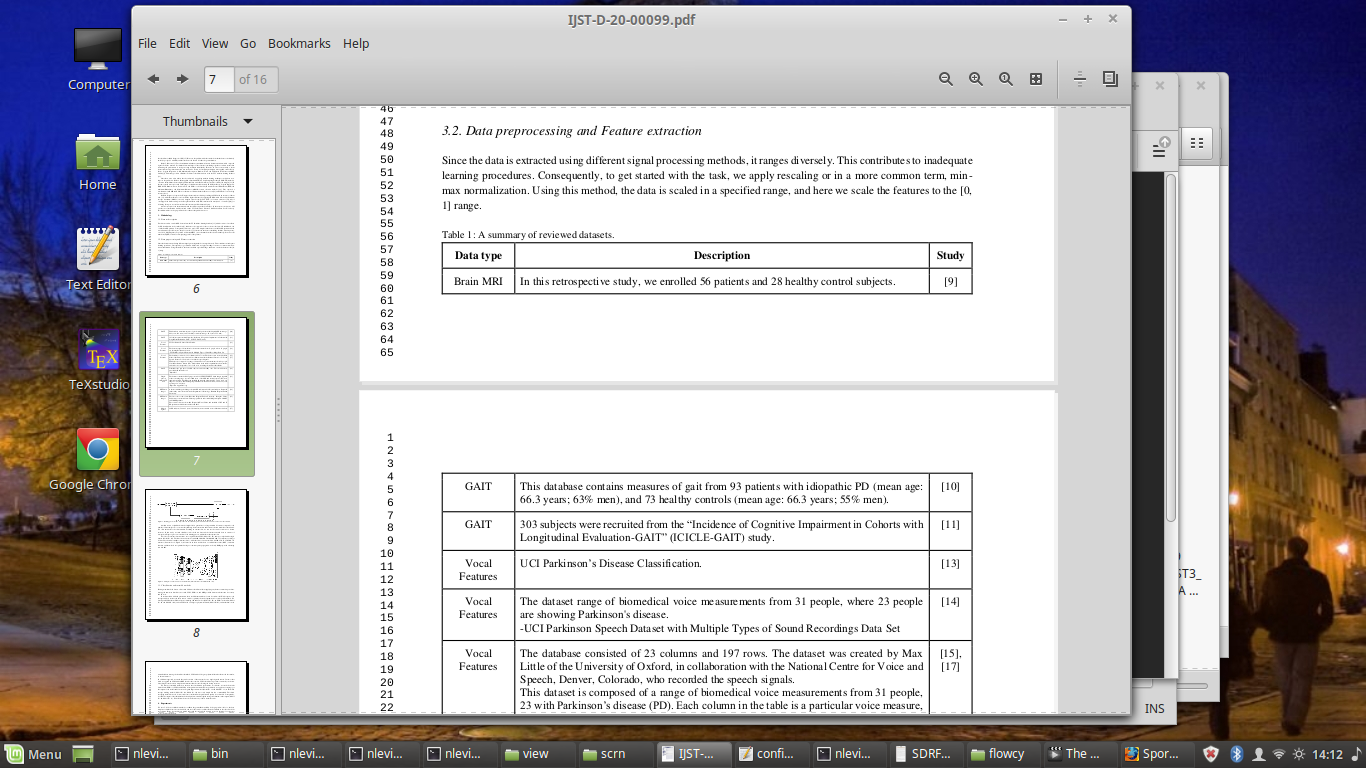
\includegraphics[trim=14cm 1.5cm 12cm 3cm,clip,width=.8\textwidth]{./scrn/s1.png}};

\rectann{darkRed}{0.7}{.5mm}{grammarArrowColor}{0.5}{4.9,-6.7}{1.5}{10.35}{1.15}

\node [anchor=west,bottom color=yellow!30!blue,top color=pink!70!green, 
inner sep=3, shading angle=50, text width=3cm]
  (longnote) at (7, 0) {\vspace{-8pt}%  %{\color{rb!85!red}{
{\cframedboxx{0mm}{2pt}{\large\raggedright\textbf{The authors provide 
citations for data sets used in their analyses ...}}}};

\end{tikzpicture}
\caption{Table Listing Analyzed Data Sets in the Parkinson's Article}
\label{fig:s1}
\end{figure}

\subsection{Unifying the Data Sets into a Single Package}  
\p{In this artice pending review, the authors summarize the data sets 
in a table within the main text 
(see Figure~\ref{fig:s1} here) and, in their bibliography, they 
cite these data sets either directly or by 
referencing publications where the relevant data sets are described 
(see Figure~\ref{fig:s2} here).  Doing so properly 
credits authorship to the researchers who curated the data sets, and it gives readers a 
means to locate the raw data.  However, accessing and working with the raw data is 
inconvenient from a reader's point of view without most or all of the data sets being 
repackaged into a \textit{single} archive that could be hosted and downloaded as one unit.  
Obtaining raw data from the resources identified in the bibliography requires 
several steps --- for instance, the PhysioNet sensor data can be downloaded 
as a zipped folder, while the demographic data attached to it has to be downloaded 
separately.  Furthermore, some of the information obtained from \MRI{} and speech analysis 
(reported in papers cited as data sources for the IJST submission) is provided 
as supplemental materials within the secondary papers; this requires readers 
to browse one at a time through each of the relevant articles so as to find 
downloadable links (see Figure~\ref{fig:s3}).  In short, piecing all 
the source data together puts the onus on readers to manually inspect multiple 
web resources and to manually interconnect files once they are downloaded.}

\p{Another complicating factor is that certain information present in the data sets 
is implicit within how the data sets are organized, requiring extra effort to 
extract this information in a machine-readable manner.  For instance, the PhysioNet 
sensor data uses a file-naming convention which encodes several pieces of 
information in the file names, such as whether the file presents a Parkinson's patient 
or a control subject (see Figure~\ref{fig:s4}).  
Though by examining file names it would be possible to construct a 
table with additional information providing context for the file contents, 
such information is not directly included within the PhysioNet data set; it 
needs to be extracted by computer code.}

\begin{figure}
\begin{tikzpicture}
\node[inner sep=0pt] (bib) at (0,0)
    {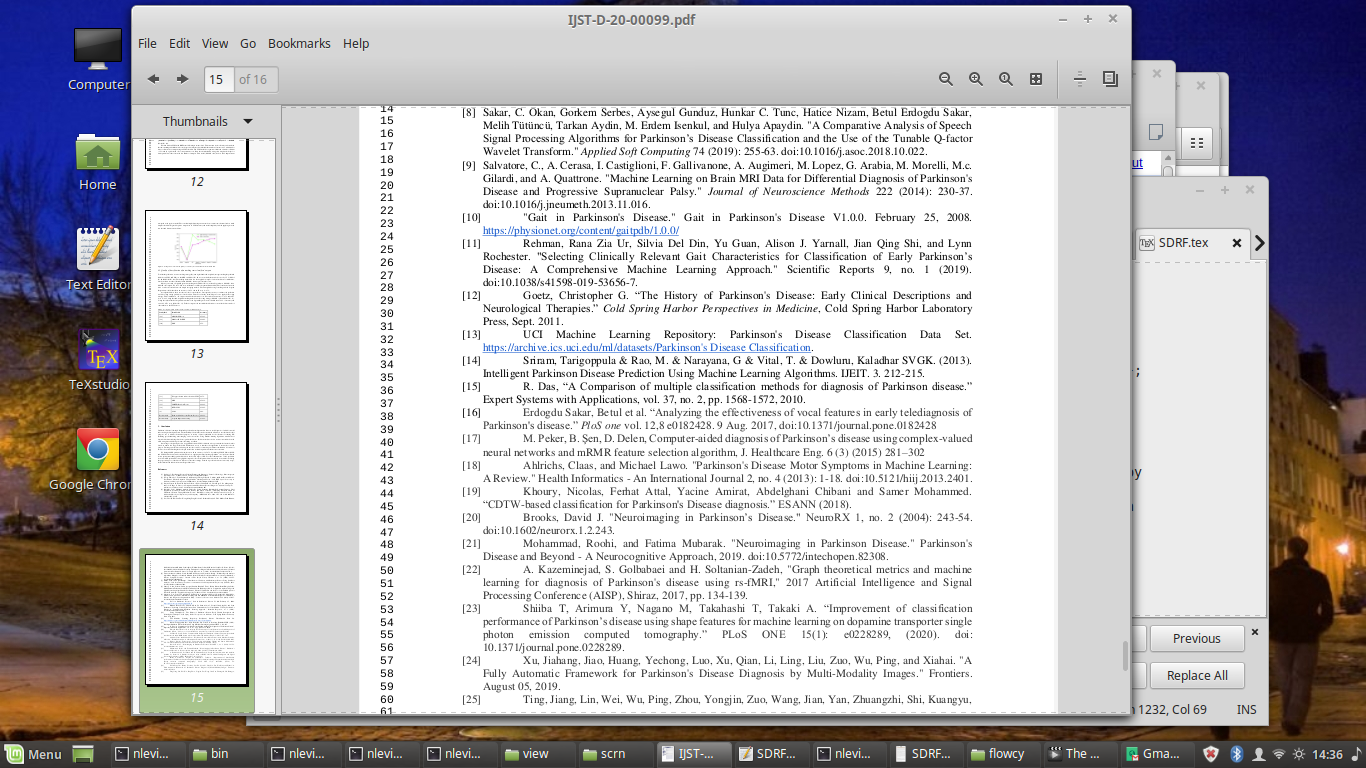
\includegraphics[trim=14cm 1.5cm 12cm 3cm,clip,width=.8\textwidth]{./scrn/s2.png}};
\ann{blue!50!orange}{1}{.6mm}{BlueGreen!90!red}{0.5}{-3.2,4.2}{2.8}{1}{1.1}
\ann{blue!50!orange}{1}{.6mm}{BlueGreen!90!red}{0.5}{-1,1.2}{5.2}{0.6}{1.1}

\colorarr{>=latex, ->}{fcBoxColor!60!black}
{0.8}{blGreen!30!red}{1}{1mm}{7.4,2.3}{4.1,1.5}

\colorarr{>=latex, ->}{fcBoxColor!60!black}
{0.8}{blGreen!30!red}{1}{1mm}{7.4,2.3}{-1.7,3.2}

\node [anchor=west,bottom color=orange!80!green,top color=pink!70!blue, 
inner sep=3, shading angle=150, text width=3cm]
  (longnote) at (7, 0) {\vspace{-8pt}%  %{\color{rb!85!red}{
{\cframedboxx{0mm}{2pt}{\large\raggedright\textbf{Some data sets 
are directly available through the bibliography; 
others have to be located by reading the cited articles.}}}};


\end{tikzpicture}
\caption{Bibliography (With Data Set Hyperrefs) in the Parkinson's Article}
\label{fig:s2}
\end{figure}

\subsection{Constructing Machine-Readable Supplemental Archives}

\p{This collection of data sets serves as an example of how technologies such 
as \SDRF{} can fill the gap between publication/data repositories and 
scientific computing, making scientific data more \q{\FAIR{}} (Findable, Accessible, 
Interoperable, Reusable).  Upon publication of this submission in 
IJST (pending peer review) the disparate open-access 
data from the article's secondary sources would be provided as a single 
\SDRF{} archive.  This archive would provide \textit{machine-readable} access to 
information spread across multiple sources, translated into a common file format.  
In general, \SDRF{} encourages and implements features to help data sets 
conform to \FAIR{} and related standards, such as (1) bundling multiple data sets 
into a single archive; (2) migrating data to general-purpose representations 
wherever possible --- formats such as \XML{}, \HDFFive{}, \ARFF{}, or 
\DICOM{}; (3) providing meta-data in multiple formats (\DCC{}, 
\textbf{schema.org/Dataset}, \MIBBI{}, \BioCoder{}, etc.) to be 
compatible with different organizations' platforms; 
(4) identifying one or more \q{preferred applications} 
for examining/reusing the published data; (5) explicitly 
representing information encoded via file-names; 
(6) bundling raw data, meta-data, and (where possible) machine-readable 
article text into a single resource, which \SDRF{} calls a 
\q{Supplemental Archive;} and (7) annnotating the data sets to support 
microcitations that granularly link the publication to its associated 
Supplemental Archive.} 

\begin{figure}
\begin{tikzpicture}
\node[inner sep=0pt] (ss) at (0,0)
    {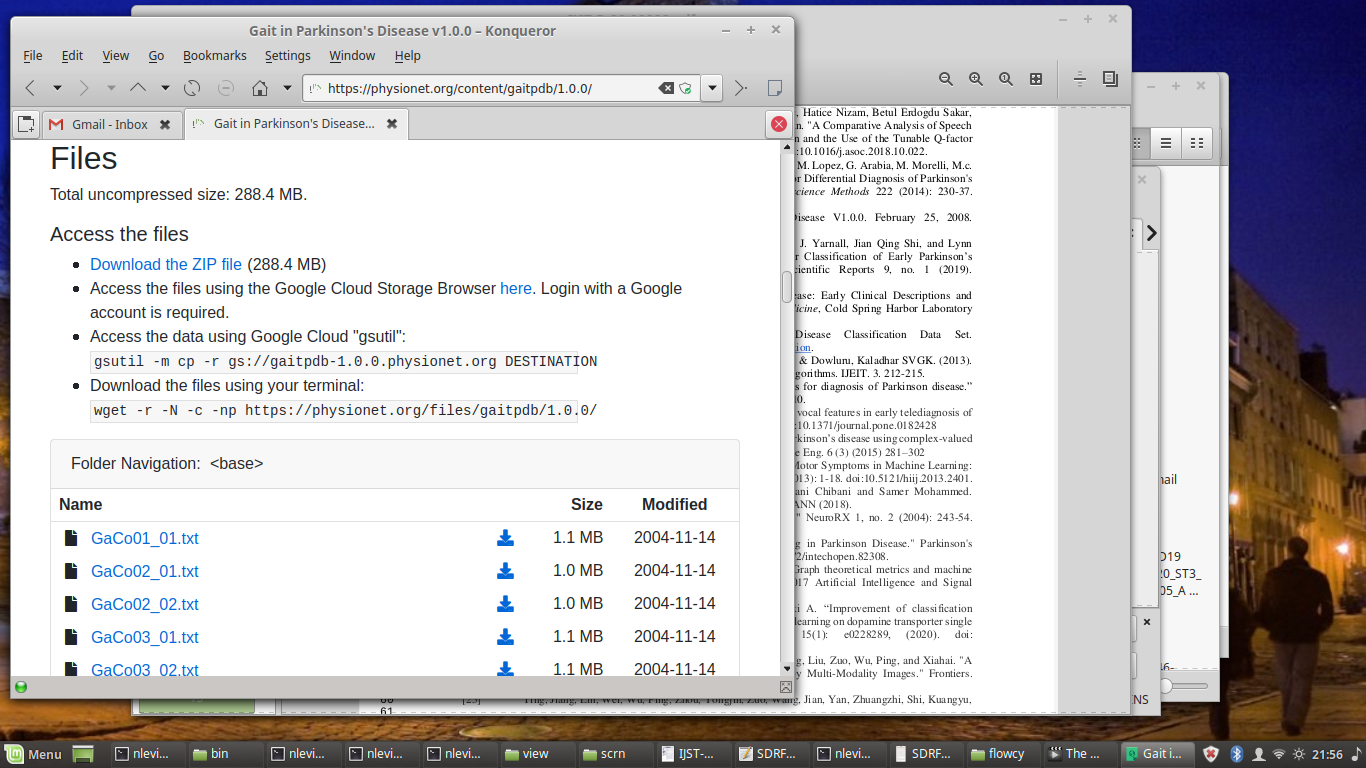
\includegraphics[trim=1cm 2cm 11cm 5cm,clip,width=.8\textwidth]{./scrn/s4.png}};
\node [anchor=west,bottom color=blGreen!80!blue,top color=green!70!blue, 
inner sep=3, shading angle=10, text width=7cm]
  (longnote) at (3.3, 0) {\vspace{-8pt}%  %{\color{rb!85!red}{
{\cframedboxx{0mm}{2pt}{\large\raggedright\textbf{Some information in 
the PhysioNet is encoded in file names, where 
the initial two letter-pairs and following two number-pairs 
all provide information about the patient and data source.  Unfortunately, 
encoding data in this manner requires extra computer code 
when reusing the data base, because the file names need 
to be analyzed so as to parse the information expressed 
via the naming conventions.}}}};

\colorarr{>=latex, ->}{blGreen!30!red}
{0.8}{blGreen!30!red}{1}{1mm}{3,-2.05}{-4.7,-2.05}

\rectann{darkRed!20!BlueGreen}{0.7}{.5mm}{BlueGreen!50!logoOrange}{2.5}{-6.8,-2.9}{5}{1.5}{1.1}

\end{tikzpicture}
\caption{Extracting Information Encoded in File Names}
\label{fig:s4}
\end{figure}


\p{Once a Supplemental Archive has been downloaded, 
an important question for any \SDRF{} archive is how researchers 
will productively access the data.  Unlike the Flow Cytometry use-case discussed below, the 
Parkinson's archive spans several scientific disciplines; as such, 
there is no obvious application which could be preferred by default 
for examining the data files.  As a fallback option, \SDRF{} is 
designed to present data sets via \Qt{} Creator, a \Cpp{} Integrated 
Development Environment associated with the \Qt{} application-development 
framework.  \lSDRF{} includes code libraries to represent 
research meta-data as \Cpp{} objects; these libraries can be 
opened as \Qt{} projects.  These may be 
supplemented with separate libraries extracting and 
managing information specific to individual data sets.  In 
particular, the Supplemental Archive for the Parkinson's 
article under peer review would provide \Cpp{} classes encapsulating spreadsheet-like 
data (whether originally in \textbf{.xls}, \CSV{}, or space-delimited formats) 
republished by the Journal in the unified data set.}

\p{An additional concern for \SDRF{} archives is how to properly annotate 
publications and data sets side-by-side.  In the Parkinson's article, 
individual \Cpp{} classes encapsulating tabular data serve as 
convenient microcitation targets: annotations within the relevant 
\Cpp{} code represent anchors through which the data set may be 
referenced (on a more precise scale than merely citing the 
Supplemental Archive as a whole).  In some places, individual 
class attributes can also be linked to lines in the authors' 
Python source code.  On the text side, certain 
paragraphs within the Parkinson's article can be linked to the 
corresponding \Cpp{} code annotations.  
This illustrates \SDRF{}'s recommended annotation/microcitation 
system, where segments in publication texts (identified for 
instance via \LaTeX{} \textbf{phantomsection} commands or 
\JATS{} \textbf{statement} tags) are linked to annotations or 
comments in code and/or raw data files in the Supplemental 
Archive.}

\begin{figure}[h]
\begin{tikzpicture}
\node[inner sep=0pt] (bib) at (0,0)
    {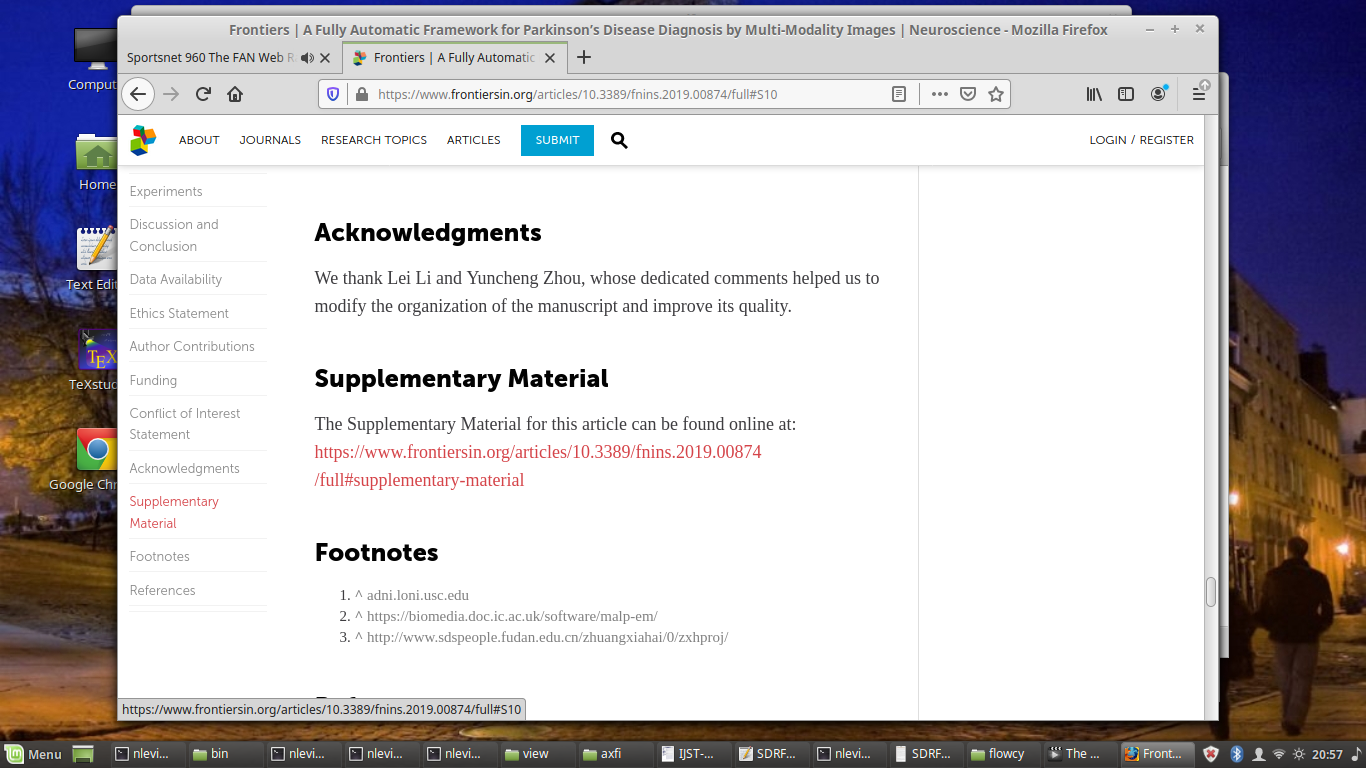
\includegraphics[trim=4cm 5cm 4.5cm 2.5cm,clip,width=.8\textwidth]{./scrn/s3.png}};
\node [anchor=west,bottom color=fcBoxColor!80!red,top color=purple!70!blue, 
inner sep=3, shading angle=10, text width=6.5cm]
  (longnote) at (4.1, -0.8) {\vspace{-8pt}%  %{\color{rb!85!red}{
{\cframedboxx{0mm}{2pt}{\large\raggedright\textbf{Some data sets 
analyzed in the Parkinson's artcle have to be located 
by browsing ``Supplemental Material'' sections of its cited papers.}}}};
\end{tikzpicture}
\caption{Indirectly Locating Data Sets from Cited Papers}
\label{fig:s3}
\end{figure}

\vspace{-12pt}
\section[Second Case Study]{\large{Second Case Study: %
\normalsize{``Marked T cell activation, senescence, exhaustion and skewing towards TH17 in patients with COVID-19 pneumonia'' from nature.com, 2020}}} 

\p{This article presents a use-case with some noteworthy contrasts to 
the Parkinson's publication described in the previous section.  This 
Covid-19 paper (\bhref{https://www.nature.com/articles/s41467-020-17292-4}) 
was published along with two data sets comprising Flow Cytometry Standard 
(\FCS{}) files hosted via the Flow Repository (\bhref{http://flowrepository.org/id/FR-FCM-Z2N4} 
and \bhref{http://flowrepository.org/id/FR-FCM-Z2N5}).  Links to the 
data sets (via \textbf{flowrepository.org} pages) are explictly provided 
in the publication's \q{Data Availability} section.  However, researchers 
still need to perform several steps to manually download the full set 
of relevant \FCS{} and meta-data files.}

\p{One feature of this second use-case is that the technical information 
in the data sets belong to a single scientific area (Flow Cytometry) 
and are mostly encoded in a single format (\FCS{}).  As such, it is 
straightforward to identify the kind of software which 
researchers need to use to visualize the raw data --- basically, any 
application that can parse \FCS{} files.  There are a variety 
of commercial as well as open-source Flow Cytometry (\FCM{}) applications 
which can be used to access \FCS{} data.  Once readers have 
downloaded the Flow Repository archives, they may individually 
load the \textbf{.fcs} files to study data which, in the 
original article, is summarized via figure illustrations.}

\p{This workflow nonetheless requires researchers to perform several 
manual steps before being able to use the published data.  The 
core problem is that existing Flow Cytometry software does not 
intrinsically have capabilities to read \PDF{} files, locate 
\FCS{} data sets, and interoperate with hosting platforms such 
as Flow Repository.  Employing this use-case as an example with 
which to illustrate proper alignment between document viewers, 
publication/data repositories, and scientific software, 
We are developing a new 
Flow Cytometry application which \textit{can} interoperate with 
\PDF{} viewers and \SDRF{} archives.  This application is 
designed so that, when authors are reading a \PDF{} file 
associated with an \FCS{} data set, the \PDF{} viewer 
can automatically launch and signal to the \FCM{} application 
when a reader wishes to download and visualize \FCS{} files.  
In short, the \FCM{} application --- having received 
data from a \PDF{} viewer which implements an 
\SDRF{} inter-application protocol --- will automatically 
execute download and extraction steps that scientists 
otherwise would have to perform manually.}

\p{Note also that, although most of the relevant 
data for this Covid-19 article is in \FCS{} form, 
there is, in addition, supplemental clinical information provided 
in other formats (...).  For cases such as these, 
the LTS \FCM{} software includes code libraries allowing 
researchers to parse non-\FCS{} data in standard 
formats such as \XML{}, \HDFFive{}, or \ARFF{}.}  
   
\p{This use-case illustrates a general principle: that 
research data is most convenient for scientists when 
it is deployed within an infrastructure where 
portals, document viewers, and scientific applications 
can seamlessly interoperate.  Wherever possible, 
when researchers are reading published books or articles, 
they should be able to \textit{automatically} launch 
the proper scientific application, download data 
sets, and examine raw data files in the preferred 
software with only one or two clicks.  These steps would be 
performed automatically as much as is feasible, 
instead of readers having to waste time with manually 
finding, downloading, merging/extracting, 
and then opening data files.}

\vspace{-6pt}
\section{Conclusion}
\p{The two case-studies considered here are similar in that 
each involve articles which are linked to multiple data sets. 
For maximum convenience, it is optimal for researchers 
to be able to access this data without performing 
manual download and merging/extracting actions.  
There are also some differences between the two 
case-studies: in particular, the 
Parkinson's data spans multiple disciplines, whereas the 
Covid-19 data is more rigorously grounded in Flow Cytometry.  
As such, the operational requirements for the Covid-19 data, 
from a reader's point of view, are more clearly delineated: 
effective integration between the publication and its 
accompanying data sets is defined by launching Flow Cytometry 
software while a researcher is reading the publication, 
allowing the researcher to view the data via software 
similar to that used to generate/analyze the data 
while the reported research was being conducted.  In 
the case of the Parkinson's data, in contrast, there is no single 
application which would seamlessly display the specrum 
of information considered in that article; as 
mentioned above, in such cases, \SDRF{} would default to using 
\Qt{} Creator as a fallback for loading Supplemental 
Archives where no other software is available.}

\p{Regardless of whether one is using \Qt{} Creator or 
a domain-specific application, 
it is preferable that each \SDRF{} archive be associated 
with one or more applications that researchers can use 
to view data (and extract information) from the archive.  
Moreover, these applications would ideally be linked 
to document viewers and also to publisher's portals, 
so that readers can automatically launch preferred 
applications and view Supplemental Archives while 
reading concomitant publications.  In order to achieve 
this, scientific applications need to be augmented 
with plugins to parse \SDRF{} data.   
To address this need, we are developing an inter-application messaging protocol 
so that disparate applications with \SDRF{} plugins 
may interoperate.  In particular, this protocol would 
entail \PDF{} viewers being able to 
interoperate with scientific applications so that 
publications' data sets may be automatically downloaded 
and visualized via the preferred software.}

\p{Our prototype example for an application utilizing such 
plugins, as mentioned above, is software for 
Flow Cytometry.  We are also working on a prototypic \Qt{} Creator 
plugin so that \Qt{} Creator (as the \q{default} \SDRF{} 
software) can participate in \SDRF{} networks using the 
same protocol.  We will then expand the scope of 
this protocol via plugins for software in other domains,  
such as image-analysis, molecular visualization, 
radiology, \ThreeD{} graphics, and so forth.}

\vspace{-6pt}
\section{Future Projections: Operationalizing SDRF}

\p{This section will present a concrete outline of the steps 
necessary to package scientific data into an \SDRF{} Supplemental 
Archive.  Data Sets may be published with content and organization 
compatible with both \SDRF{} and other formats, such as 
Research Object Bundles, so using \SDRF{} does not preclude 
adopting other formats as well.  For example, a data set which 
provides \SDRF{} meta-data may also include the \textbf{meta-inf} 
files required by Research Objects.  Indeed, it is recommended 
that authors aim for compatibility with multiple standards, 
not only \SDRF{}.  This section, however, will focus on the 
components of Supplemental Archives that are specific to \SDRF{}.}

\p{This section will describe two different approaches to 
using \SDRF{}.  One approach employs \SDRF{} to a limited 
extent, deferring to older technologies for such basic 
operations as encoding data or annotating publications.  
An alternative is to adopt \SDRF{} more holistically, 
adopting experimental or under-development features in the 
\SDRF{} libraries.  When discussed in the following 
outline, these features will usually be characterized 
as \q{experimental} or \q{specific to \SDRF{} code libraries.}}

\subsection{Formulating Scientific Data Repository Models 
for Individual Publishing Environments}

\p{\lSDRF{} is intended to interoperate with mulitple 
publisher and data-hosting platforms, each of which have 
their own requirements and technology.  Therefore, the 
precise contents and organization of a given \SDRF{} 
Supplemental Archive will depend on specifications 
pertaining the specific repository and hosting platform 
where the publication and data set, respectively, 
are to be deposited.  To facilitate Supplemental Archive 
preparation for different environments, \SDRF{} 
seeks to include \q{Scientific Data Repository Models} 
(\SDRM{}s) which are tailored to individual publishers.  
The \SDRM{}s would encapsulate information pertaining 
to the specific platforms where the relevant publication 
and data set are hosted.  For example, research 
funded by the Bill and Melinda Gates Foundation 
must follow certaing guidelines, which are 
documented whenever an article is submitted to the 
Gates Open Research portal.  Consequently, the 
specific \SDRF{} meta-data for such papers can 
be designed to notate the concordant research's 
adherence to these organizational guidelines.  
In these situations, the layout and vocabulary 
for \SDRF{} meta-data would be determined 
at least in part by the \SDRM{} germane 
to the environment where the research is published.}

\p{The purpose of an \SDRM{} is also to facilitate 
the implementation of technologies which interoperate 
with publishers' platforms --- for instance, 
\API{} clients which can request information from 
document/data portals (e.g., locating articles 
or data sets via keywork searches), or 
\PDF{} viewers enhanced with capabilities to 
obtain data sets from hosting platforms 
(to automatically download data sets upon 
request from a user reading the corresponding publication).  
For these use-cases, individual \SDRM{} would 
include information and/or computer code about 
how to access publishers' \API{}s, how to download 
and extract a data set given a digital identifier, 
and so forth.}

\p{Because \SDRF{} Supplemental Archives may differ somewhat 
according to the specific \SDRM{} in effect, any 
description of these archives is provisional.  To be 
precise, \SDRF{} assumes a generic \SDRM{} --- 
dubbed \q{\MOSAIC{}} --- which can be extended 
or modified in consultation with individual 
publishers, as required.  As such, the following 
outline will apply intrinsically to the 
\MOSAIC{} \SDRM{}; depending on the platform, 
the details for individual \SDRF{} Supplemental Archives may 
be different than the generic model presented here.}

\subsection{Standard Components of SDRF Supplemental Archives}

\p{The components of an \SDRF{} Supplemental Archive can be 
grouped into several facets, concerning meta-data, raw data, and 
machine-readable text, respectively.

\begin{enumerate}

\item{} \textbf{SDRF Meta-Data}
\begin{description}
\item[Meta-Data Files]  \SDRF{} uses a vocabulary for 
describing the contents of data sets which merges the 
data models of several existing formats, such as 
\DCC{} and \textbf{schema.org/Dataset}.  \SDRF{} 
recommends encoding this data in \TAGML{} 
(\q{Text-as-Graph Markup Language}), which is a very flexible, 
and computationally powerful representation 
format.\footnote{\sTAGML{} is \q{powerful} in the 
sense that, with suitable mappings between their 
disparate syntactic expressions, \sTAGML{} represents 
a superset of \sXML{} and other common data-representation 
languages, such as \sJSON{}.}  The \SDRF{}-specific 
libraries include parsers for (an extended version of) \TAGML{}.  

\item[C++ Files]  \SDRF{} also recommends that authors provide 
\Cpp{} code to initialize objects representing Supplemental 
Archive's meta-data.  These objects may be directly constructed 
from the \TAGML{} meta-data files, or authors may choose to 
customize the \Cpp{} logic as desired.  For lab-based research, 
authors may employ \BioCoder{}, which uses \Cpp{} code to 
notate research protocols and workflows (the \SDRF{} libraries 
include a modified version of \BioCoder{}).  Moreover, 
for data sets whose \q{preferred application} for opening 
raw data files is implemented in \Cpp{} (as is the case 
for many, if not most, scientific-computing applications), 
the Supplemental Archive may include plugins or extensions 
to these applications.  In general, using \Cpp{} objects 
specific to Supplemental Archive meta-data as a basis, 
authors (or programmers coding on authors' behalf) may 
introduce additional \Cpp{} code demonstrating or 
enabling analysis, visualization, or application-integration 
for the Supplemental Archive's raw data.

\item[SDRM-Specific Meta-Data]  Either via data files or 
computer code, information or capabilities specific 
to the platforms where papers and Supplemental Archives 
are hosted may be presented in conjunction with 
the applicable \SDRM{}s.  For instance, \Cpp{} code 
distributed with the archive may include 
procedures for accessing \API{}s of the hosting service 
where the archive is deposited.   

\item[Qt Project Files]   As explained earlier, 
\SDRF{} defaults to using \Qt{} Creator as an application 
with which to examine data sets, if there is no 
obvious \q{preferred application} based on the research 
topic.  Therefore, \SDRF{} recommends that the \Cpp{} 
meta-data code be paired with \Qt{} project files and 
other assets needed to run the code in the \Qt{} Creator 
Integrated Development Environment, using \textbf{qmake} 
as the build system.  In general, there should be 
a \Qt{} project specific to the \SDRF{} meta-data; 
in some cases, there will also be separate 
\Qt{} projects for working with raw data files.
\end{description}

\item{} \textbf{Raw Data}:  As mentioned above, \SDRF{} 
recommends that raw data be encoded in general-purpose 
formats such as \ARFF{}, \HDFFive{}, \XML{}, or 
\TAGML{} (as compared to formats such as 
\textbf{.xls}, which are associated with specific 
applications).  An experimental \q{Hypergraph 
Exchange Format} (\HGXF{}) may also be used.

An exception to the guidelines for general-purpose 
formats is when data should be presented in 
optimized formats endemic to a certain scientific 
field, such as \FCS{} files for Flow Cytometry, 
or \DICOM{} files for bioimaging.  In these cases, 
it is recommended to employ such formats for most 
of the raw data files but also to construct summaries 
of the data, which may facilitate properly loading 
and accessing the domain-specific files, represented 
in a more general-purpose format.    

\item{} \textbf{Annotated Manuscripts}  Where authors have permission 
to share full-text versions of their books/articles, \SDRF{} 
recommends that a machine-readable representation of 
these publications, in formats such as \TAGML{} or 
\XML{}, be included in the Supplemental Archive 
(\SDRF{} has an experimental \q{Hypergraph 
Text Encoding Protocol} which may be utilized as well).  
This machine-readable manuscript may then be 
annotated and cross-referenced with raw data and/or 
code files also included in the Supplemental Archive.  
An experimental \SDRF{} \LaTeX{} package provides 
an annotation framework which not only marks locations 
in document text, but also encodes \PDF{} viewport 
coordinates for use by specialized \PDF{} viewers 
which implement an \SDRF{} protocol for integrating 
\PDF{} viewers with scientific applications.
\end{enumerate}
}

\section{Checklist for Authors, Editors, and Publishers}
\p{To clarify the steps needed to deploy publications 
and data steps according to \SDRF{} recommendations, 
this section will outline the steps that would be 
taken by individuals fulfilling different roles in 
the publishing pipeline.

\begin{description}

\item[Authors]  In most publishing environments, 
the process of depositing data sets for open-access  
hosting is entirely separate from that of submitting 
articles for peer-reviewed publication.  Therefore, 
it is the responsibility of authors to ensure that 
these two resources --- their manuscripts and 
Supplemental Archives --- are properly interconnected.  
Some guidelines for ensuring that this process is 
carried out smoothly include: (1) site the 
\URL{} for the data set near the top of the document; 
(2) cite the \URL{} for the publication in a 
\textbf{readme} or similarly prominent 
location in the data set; (3) if there are no 
access restrictions, include a \PDF{} file 
showing the full article in a findable location in 
the data set; (4) use labels and \textbf{phantomsection} 
or similar tags/commands to mark locations in the 
manuscript which are conceptually linked to parts of 
the data set; and (5) request that future authors 
cite both the publication \URL{} and the Supplemental Archive 
\URL{} when referencing the body of research.

Additional steps are necessary when packaging files into 
the published archive.  The exact details will depend 
on the \SDRM{}s which apply to the environments 
where the publication and data set are hosted, and 
also on whether authors wish to comply with research 
standardizations other than those of \SDRF{}.  For 
example, archives which are published as a 
Research Object Bundle need to use a folder layout 
proscribed by that specification.  To work flexibly 
with other standards, \SDRF{} does not demand 
\textit{a priori} that authors use specific conventions 
for file and folder names and hierarchies.  In general, 
so as to pin the location of \SDRF{} meta-data, 
\SDRF{} recommends the following: \Cpp{} classes and 
\textbf{main.cpp} files specific to initializing 
\SDRF{} meta-data should be marked accordingly with 
\Cpp{} comments; and files in formats such as 
\TAGML{}, serializing \SDRF{} meta-data, should 
be similarly identified.  Once the meta-data source is 
locatable within the archive, all other information 
needed to fully parse the \SDRF{}-specific data 
should be extracted from the initialized meta-data objects.  

\item[Editors]  Because (as just outlined) authors' submissions 
to data-hosting portals are usually operationally separate 
from their endeavors to publish books and articles, publication 
editors ordinarily cannot directly influence the authors' 
preparations for publishing their data sets.  However, 
editors can make recommendations and double-check that 
their own research (and other research which is cited 
within the article) is properly referenced, ensuring 
that new (and relevant pre-existing) data sets are 
Findable.  That is, editors can ensure that (1) \URL{}s 
and digital identifiers for concomitant are prominently 
notated in the publication text; (2) bibliographic 
references to other publications linked to their own 
data sets include citations for and hyperref links to 
those resources if possible; and (3) the authors provide 
a brief overview of their data set if that is necessary 
to help researchers access the raw data and to help 
readers understand how the raw data has informed the 
research or findings presented in the publication.  
Moreover, editors can access the data sets directly 
through their hosting portals (or, for data sets 
still in preparation, request access to the raw data 
from the authors) and verify that the data set 
properly references the accompanying publication. 

It should be noted that the proper \URL{} and format 
for referencing publications may change as manuscripts 
work their way through the publishing process.  
For example, a web link for accessing a peer-reviewed 
article may only be defined once the document is 
accepted for publication.  Also, some institutions 
--- again, Gates Open Research supplies an example --- 
explicitly track a submission through different stages 
of peer review (articles may be accessible for reading 
even while they are still being reviewed or 
finalized).  When a data set links to its accociated 
publication, then, such information about the current 
state of the submission should be duly observed in the 
data set.

In short, the precise publication-related data within a 
Supplemental Archive may need to be modified one 
or more times as a document submission is processed, 
so editors should be prepared to notify authors when 
a change within the data set is necessary.

\item[Publishers]  Assuming that authors and 
editors follow the steps just outlined, 
articles and Supplemental Archives may be 
published in any environment without altering 
publishers' workflows or technologies.  
However, their are steps which publishers 
may take to enhance the usefulness of \SDRF{} 
resources, and to derive additional scientific 
and commercial value from hosting articles 
that utilize \SDRF{}.  These steps include:

\begin{itemize}
\item{} \textbf{Feature Data-Set References on Article 
Front Pages}  The \q{front page} of an article is 
\URL{} which uniquely locates a given publication on a 
publisher's portal.  Usually this front page includes 
an abstract, bibliographic citations, author names/affiliations, 
keywords, and other high-level info about the document; 
in some environments, the front-page also reproduces the 
full text of the article (usually in \HTML{} format).  
Even with this information set forth, however, it 
can be difficult for readers to identify which publications 
are paired with open-access data sets and to locate 
those data sets when they are available.  Publishers 
can rectify this situation by including links 
to data sets near the top of the front page.

\item{} \textbf{Recognize Data-Set Microcitations in Manuscripts}  
Properly connecting publications and data sets requires 
customized \LaTeX{} commands or \XML{} attributes, so as 
to mark and annotate relevant locations/passages within the 
document.  To fully utilize \SDRF{}, then --- or, indeed, 
any rigorous data-sharing protocol --- publishers need to 
expand their in-house media for internally representing 
manuscripts in the pipeline with a collection of 
additional tags, commands, and/or attributes.  The 
details of these add-ons, depending on the technology 
used, may be codified within individual \SDRM{}s.

\item{} \textbf{Recognize Alternative Manuscript and 
\PDF{} Formats}  This applies to non-restricted publications 
where full text representations may be included within 
Supplemental Archive.  In this situation, the ideal  
\PDF{} version of a document, as well as the machine-readable 
encoding of the text, may be different from what is 
internally used by the publisher.  For example, 
an article may appear as a chapter in a book, typeset 
according to the book's conventions; in the data set, 
however, that same article is shared as its own 
document, and might use different typesetting rules 
optimized for its specific content.  Also, the 
machine-readable full-text representations presented 
in the data set should be optimized for Text and Data 
Mining (\TDM{}), and may therefore differ from the 
internal encoding used by the publisher.  For these 
scenarios, publishers should allow for alternate 
versions of both human-readable and machine-readable 
publication text being incorporated into the publishing 
process, where these alternatives end up becoming 
assets within Supplemental Archives.  Such alternatives 
may not differ in terms of textual content 
(although a data-set-specific version of an article 
may include supplemental instructions for using the data set), 
but they can differ in the visual formatting of the text 
as well as how the text is encoded. 

\item{} \textbf{Register Cross-References Between Publications and 
Data Sets}  Publishers' databases should be configured to 
clearly designate when a publication is linked to an 
associated data set.  Moreover, some third-party 
biblioinformatics services, such as CrossRef, allow 
publishers to introduce additional attributes describing 
publications.  Connections between publications and 
data sets may therefore be formally declared in these 
third-party contexts.

\item{} \textbf{Incorporate Data-Sets Information into Publisher APIs}
Most publishing portals use \API{}s to support application-level 
queries for finding or accessing publications.  These \API{}s 
can be extended to systematically honor associations between 
publications and data sets, e.g.: (1) return the \URL{} for a 
data set when given an article's Document Object Identifier; 
(2) return information about an article when queried by a 
software component designed to manage data sets; (3) search 
for publications whose data sets fit given criteria 
(file format, programming language, subject area, etc.); and 
(4) given a publication, return basic information about its associated 
data that may help a reader decide whether to 
download the data set (file format, total file size, preferred application, 
etc.).     
\end{itemize}
\end{description}
}

\subsection{Benefits for Publishers}
\p{We believe adopting \SDRF{} technology can derive several 
benefits for publishers (as well as instutions, such as 
universities or independent journals, which publish their 
own material).  Bear in mind that the details are \SDRF{} 
are adapted to different \SDRM{}s; therefore, the characterization 
of \SDRF{} content presented here is provisional, and may 
take different forms in different publishing environments.  
Therefore, adopting \SDRF{} does not require publishers 
to substantially (or at all) modify their existing software.  
In general, though, incorporating certain \SDRF{} 
protocols and/or implementations --- whether as software 
extensions or simply as recommended design patterns --- 
can augment publishers' offerings in several ways:

\begin{enumerate}
\item{}  \textbf{Increased Citations and Downloads}  By 
explicitly linking publications and data sets, publishers 
improve the likelihood that researchers will find 
the publications.  Data sets present an alternative 
route (alongside references in other sources, or 
keywork searches) for scholars to locate books and 
articles relevant to their research.  

It is important to stress that, despite standardizations 
such as \DCC{} and Research Objects, the vast majority of 
published data sets are shared haphazardly, without 
proper organization or meta-data.  Therefore, those 
data-sets which \textit{do} adopt rigorous curation 
standards are more likely to be found by software 
designed for contemporary data-publishing specifications.  
These well-curated resources may also stand out from their 
peers on data hosting platforms.  Some hosting environments 
explicitly introduce a \q{score} to measure how well 
each data set is organized and documented (e.g., 
the \MIFlowCyt{}, or \q{Minimumum Information about a 
Flow Cytometry Experiment}, rating on \textbf{flowRepository.org}).  
Accordingly, data sets which score highly on existing or 
future metrics --- 
assessing how systematically their data is organized --- 
are more likely to attract researchers' attention, which 
in turn drives traffic to the publication sites where 
data sets' corresponding articles are indexed. 
   
\item{}  \textbf{Impact Factor}  Articles which are 
paired with conscientiously curated, well-documented 
and reusable data sets are more likely to 
spur further research than publications whose raw 
data is not shared at or is shared in ways which 
add extra effort for researchers seeking to re-use 
or re-examine the data.  In general, scientists 
grivitate to using raw data which can be plugged 
most readily into the computing environments they 
use for their own research.  For this reason, 
research work --- expressed both in data sets and 
in publications discussing the research --- is 
likely to be more influential when scientists 
deem the data convenient to use and expand upon.  

\item{}  \textbf{Enhancing the Publishing Ecosystem}  
As digital media becomes an increasingly important part 
of scientist's use and experience of published research, 
publishers are expected to provide ever more sophisticated 
technology for visualizing data and publications.  
Aside from just showing \PDF{} or \HTML{} views of 
articles, publishers are gradually introducing 
multi-media platforms which permit interactive 
data access, \ThreeD{} data visualization, 
audio and video content, and so forth.  Interfacing 
directly with scientific applications --- e.g., 
via publisher-specific application plugins --- 
is a natural corrolary to this trend, adding yet 
more computational heft to publishers' platforms.  
But properly networking publications with 
specific software demands rigorously documented 
links between publications and data sets, such as 
provided via \SDRF{}.   
\end{enumerate}
}

\section{The Transparent Hypergraph Query Language}
\p{\lSDRF{} does not overtly proscribe any particular 
format for encoding raw data in \SDRF{} archives; 
as such, \SDRF{} cannot make definitive recommendations 
for how this data may be consumed.  Nevertheless, 
\SDRF{} draws on contemporary research into database 
engineering, particularly the body of literature 
concerning Hypergraph Database design and the 
use of hypergraphs as multi-faceted, general-purpose 
formats for representing information.  Hypergraph 
Database engines are favored in part because hypergraph 
schema can incorporated many families of data models, 
so that Hypergraph Databases can store diverse, heterogeneous 
data, sourced from disparate origin-points.}

\p{Nevertheless --- despite some common features which make Hypergraph Database 
engines, collectively, good architectural choices 
for heterogeneous and decentralized data persistence ---  
there are several distinct Hypergraph engines 
widely used in contemporary technology, each with slightly 
different data models and protocols.  It is therefore a 
worthwhile project to define a multi-purpose Hypergraph data 
model which merges idiosyncratic details of 
these various platforms, offering a common framework for 
accessing Hypergraph data.  Such a frameworks' value could 
be enhanced by applying it to information spaces which 
are not, necessarily, backed by a Hypergraph Database engine 
but which are amenable to an intermediate software layer which 
translates Hypergraph-oriented queries to a query language 
endemic to the actual database used.  Although Hypergraph databases 
are gaining a greater foothold in some computing domains 
(biomedical, governmental, financial, etc.), a much larger 
proportion of database instances rely on more traditional 
data-storage technology.   With proper software 
adapters, it is possible to construct \q{views} onto 
data spaces such that they can be operationally interacted 
with as if they employed hypergraph models internally.}

\p{These points apply not only to databases themselves 
but also to any systematic data compilation, including 
published data sets.  Therefore, one use-case for 
\SDRF{} is to package raw data in such a way that 
it may be queried according to protocols established 
for Hypergraph Database engines and then extended 
to other information architectures.}

%impact factor

%\p{}
}
\end{document}



